\documentclass[twoside]{book}

% Packages required by doxygen
\usepackage{fixltx2e}
\usepackage{calc}
\usepackage{doxygen}
\usepackage[export]{adjustbox} % also loads graphicx
\usepackage{graphicx}
\usepackage[utf8]{inputenc}
\usepackage{makeidx}
\usepackage{multicol}
\usepackage{multirow}
\PassOptionsToPackage{warn}{textcomp}
\usepackage{textcomp}
\usepackage[nointegrals]{wasysym}
\usepackage[table]{xcolor}

% Font selection
\usepackage[T1]{fontenc}
\usepackage[scaled=.90]{helvet}
\usepackage{courier}
\usepackage{amssymb}
\usepackage{sectsty}
\renewcommand{\familydefault}{\sfdefault}
\allsectionsfont{%
  \fontseries{bc}\selectfont%
  \color{darkgray}%
}
\renewcommand{\DoxyLabelFont}{%
  \fontseries{bc}\selectfont%
  \color{darkgray}%
}
\newcommand{\+}{\discretionary{\mbox{\scriptsize$\hookleftarrow$}}{}{}}

% Page & text layout
\usepackage{geometry}
\geometry{%
  a4paper,%
  top=2.5cm,%
  bottom=2.5cm,%
  left=2.5cm,%
  right=2.5cm%
}
\tolerance=750
\hfuzz=15pt
\hbadness=750
\setlength{\emergencystretch}{15pt}
\setlength{\parindent}{0cm}
\setlength{\parskip}{3ex plus 2ex minus 2ex}
\makeatletter
\renewcommand{\paragraph}{%
  \@startsection{paragraph}{4}{0ex}{-1.0ex}{1.0ex}{%
    \normalfont\normalsize\bfseries\SS@parafont%
  }%
}
\renewcommand{\subparagraph}{%
  \@startsection{subparagraph}{5}{0ex}{-1.0ex}{1.0ex}{%
    \normalfont\normalsize\bfseries\SS@subparafont%
  }%
}
\makeatother

% Headers & footers
\usepackage{fancyhdr}
\pagestyle{fancyplain}
\fancyhead[LE]{\fancyplain{}{\bfseries\thepage}}
\fancyhead[CE]{\fancyplain{}{}}
\fancyhead[RE]{\fancyplain{}{\bfseries\leftmark}}
\fancyhead[LO]{\fancyplain{}{\bfseries\rightmark}}
\fancyhead[CO]{\fancyplain{}{}}
\fancyhead[RO]{\fancyplain{}{\bfseries\thepage}}
\fancyfoot[LE]{\fancyplain{}{}}
\fancyfoot[CE]{\fancyplain{}{}}
\fancyfoot[RE]{\fancyplain{}{\bfseries\scriptsize Generated by Doxygen }}
\fancyfoot[LO]{\fancyplain{}{\bfseries\scriptsize Generated by Doxygen }}
\fancyfoot[CO]{\fancyplain{}{}}
\fancyfoot[RO]{\fancyplain{}{}}
\renewcommand{\footrulewidth}{0.4pt}
\renewcommand{\chaptermark}[1]{%
  \markboth{#1}{}%
}
\renewcommand{\sectionmark}[1]{%
  \markright{\thesection\ #1}%
}

% Indices & bibliography
\usepackage{natbib}
\usepackage[titles]{tocloft}
\setcounter{tocdepth}{3}
\setcounter{secnumdepth}{5}
\makeindex

% Hyperlinks (required, but should be loaded last)
\usepackage{ifpdf}
\ifpdf
  \usepackage[pdftex,pagebackref=true]{hyperref}
\else
  \usepackage[ps2pdf,pagebackref=true]{hyperref}
\fi
\hypersetup{%
  colorlinks=true,%
  linkcolor=blue,%
  citecolor=blue,%
  unicode%
}

% Custom commands
\newcommand{\clearemptydoublepage}{%
  \newpage{\pagestyle{empty}\cleardoublepage}%
}

\usepackage{caption}
\captionsetup{labelsep=space,justification=centering,font={bf},singlelinecheck=off,skip=4pt,position=top}

%===== C O N T E N T S =====

\begin{document}

% Titlepage & ToC
\hypersetup{pageanchor=false,
             bookmarksnumbered=true,
             pdfencoding=unicode
            }
\pagenumbering{alph}
\begin{titlepage}
\vspace*{7cm}
\begin{center}%
{\Large My Project }\\
\vspace*{1cm}
{\large Generated by Doxygen 1.8.14}\\
\end{center}
\end{titlepage}
\clearemptydoublepage
\pagenumbering{roman}
\tableofcontents
\clearemptydoublepage
\pagenumbering{arabic}
\hypersetup{pageanchor=true}

%--- Begin generated contents ---
\chapter{Todo List}
\label{todo}
\Hypertarget{todo}

\begin{DoxyRefList}
\item[\label{todo__todo000001}%
\Hypertarget{todo__todo000001}%
Member \mbox{\hyperlink{classnews_1_1models_1_1_blog_a5cf49bbf405b3dfcbbe79905827ee3e7}{news.models.Blog.\+\_\+\+\_\+str\+\_\+\+\_\+}} (self)]Дописать пару функций 

Протестить
\end{DoxyRefList}
\chapter{Bug List}
\label{bug}
\Hypertarget{bug}

\begin{DoxyRefList}
\item[\label{bug__bug000001}%
\Hypertarget{bug__bug000001}%
Member \mbox{\hyperlink{classnews_1_1models_1_1_blog_a5cf49bbf405b3dfcbbe79905827ee3e7}{news.models.Blog.\+\_\+\+\_\+str\+\_\+\+\_\+}} (self)]Описание бага 
\end{DoxyRefList}
\chapter{Namespace Index}
\section{Namespace List}
Here is a list of all namespaces with brief descriptions\+:\begin{DoxyCompactList}
\item\contentsline{section}{\mbox{\hyperlink{namespacenews}{news}} }{\pageref{namespacenews}}{}
\item\contentsline{section}{\mbox{\hyperlink{namespacenews_1_1admin}{news.\+admin}} }{\pageref{namespacenews_1_1admin}}{}
\item\contentsline{section}{\mbox{\hyperlink{namespacenews_1_1apps}{news.\+apps}} }{\pageref{namespacenews_1_1apps}}{}
\item\contentsline{section}{\mbox{\hyperlink{namespacenews_1_1migrations}{news.\+migrations}} }{\pageref{namespacenews_1_1migrations}}{}
\item\contentsline{section}{\mbox{\hyperlink{namespacenews_1_1migrations_1_10001__initial}{news.\+migrations.\+0001\+\_\+initial}} }{\pageref{namespacenews_1_1migrations_1_10001__initial}}{}
\item\contentsline{section}{\mbox{\hyperlink{namespacenews_1_1migrations_1_10002__auto__20181009__2006}{news.\+migrations.\+0002\+\_\+auto\+\_\+20181009\+\_\+2006}} }{\pageref{namespacenews_1_1migrations_1_10002__auto__20181009__2006}}{}
\item\contentsline{section}{\mbox{\hyperlink{namespacenews_1_1migrations_1_10003__text}{news.\+migrations.\+0003\+\_\+text}} }{\pageref{namespacenews_1_1migrations_1_10003__text}}{}
\item\contentsline{section}{\mbox{\hyperlink{namespacenews_1_1migrations_1_10004__delete__text}{news.\+migrations.\+0004\+\_\+delete\+\_\+text}} }{\pageref{namespacenews_1_1migrations_1_10004__delete__text}}{}
\item\contentsline{section}{\mbox{\hyperlink{namespacenews_1_1migrations_1_10005__blog}{news.\+migrations.\+0005\+\_\+blog}} }{\pageref{namespacenews_1_1migrations_1_10005__blog}}{}
\item\contentsline{section}{\mbox{\hyperlink{namespacenews_1_1migrations_1_10006__auto__20181013__0120}{news.\+migrations.\+0006\+\_\+auto\+\_\+20181013\+\_\+0120}} }{\pageref{namespacenews_1_1migrations_1_10006__auto__20181013__0120}}{}
\item\contentsline{section}{\mbox{\hyperlink{namespacenews_1_1migrations_1_10007__auto__20181013__0120}{news.\+migrations.\+0007\+\_\+auto\+\_\+20181013\+\_\+0120}} }{\pageref{namespacenews_1_1migrations_1_10007__auto__20181013__0120}}{}
\item\contentsline{section}{\mbox{\hyperlink{namespacenews_1_1models}{news.\+models}} }{\pageref{namespacenews_1_1models}}{}
\item\contentsline{section}{\mbox{\hyperlink{namespacenews_1_1serializers}{news.\+serializers}} }{\pageref{namespacenews_1_1serializers}}{}
\item\contentsline{section}{\mbox{\hyperlink{namespacenews_1_1tests}{news.\+tests}} }{\pageref{namespacenews_1_1tests}}{}
\item\contentsline{section}{\mbox{\hyperlink{namespacenews_1_1translation}{news.\+translation}} }{\pageref{namespacenews_1_1translation}}{}
\item\contentsline{section}{\mbox{\hyperlink{namespacenews_1_1views}{news.\+views}} }{\pageref{namespacenews_1_1views}}{}
\end{DoxyCompactList}

\chapter{Hierarchical Index}
\section{Class Hierarchy}
This inheritance list is sorted roughly, but not completely, alphabetically\+:\begin{DoxyCompactList}
\item \contentsline{section}{news.\+serializers.\+Blog\+Serializer.\+Meta}{\pageref{classnews_1_1serializers_1_1_blog_serializer_1_1_meta}}{}
\item Migration\begin{DoxyCompactList}
\item \contentsline{section}{news.\+migrations.0001\+\_\+initial.Migration}{\pageref{classnews_1_1migrations_1_10001__initial_1_1_migration}}{}
\item \contentsline{section}{news.\+migrations.0002\+\_\+auto\+\_\+20181009\+\_\+2006.Migration}{\pageref{classnews_1_1migrations_1_10002__auto__20181009__2006_1_1_migration}}{}
\item \contentsline{section}{news.\+migrations.0003\+\_\+text.Migration}{\pageref{classnews_1_1migrations_1_10003__text_1_1_migration}}{}
\item \contentsline{section}{news.\+migrations.0004\+\_\+delete\+\_\+text.Migration}{\pageref{classnews_1_1migrations_1_10004__delete__text_1_1_migration}}{}
\item \contentsline{section}{news.\+migrations.0005\+\_\+blog.Migration}{\pageref{classnews_1_1migrations_1_10005__blog_1_1_migration}}{}
\item \contentsline{section}{news.\+migrations.0006\+\_\+auto\+\_\+20181013\+\_\+0120.Migration}{\pageref{classnews_1_1migrations_1_10006__auto__20181013__0120_1_1_migration}}{}
\item \contentsline{section}{news.\+migrations.0007\+\_\+auto\+\_\+20181013\+\_\+0120.Migration}{\pageref{classnews_1_1migrations_1_10007__auto__20181013__0120_1_1_migration}}{}
\end{DoxyCompactList}
\item Model\begin{DoxyCompactList}
\item \contentsline{section}{news.\+models.\+Article}{\pageref{classnews_1_1models_1_1_article}}{}
\item \contentsline{section}{news.\+models.\+Blog}{\pageref{classnews_1_1models_1_1_blog}}{}
\end{DoxyCompactList}
\item Model\+Serializer\begin{DoxyCompactList}
\item \contentsline{section}{news.\+serializers.\+Blog\+Serializer}{\pageref{classnews_1_1serializers_1_1_blog_serializer}}{}
\end{DoxyCompactList}
\item Model\+View\+Set\begin{DoxyCompactList}
\item \contentsline{section}{news.\+views.\+Blog\+View\+Set}{\pageref{classnews_1_1views_1_1_blog_view_set}}{}
\end{DoxyCompactList}
\item App\+Config\begin{DoxyCompactList}
\item \contentsline{section}{news.\+apps.\+News\+Config}{\pageref{classnews_1_1apps_1_1_news_config}}{}
\end{DoxyCompactList}
\item Translation\+Admin\begin{DoxyCompactList}
\item \contentsline{section}{news.\+admin.\+Blog\+Admin}{\pageref{classnews_1_1admin_1_1_blog_admin}}{}
\item \contentsline{section}{news.\+admin.\+News\+Admin}{\pageref{classnews_1_1admin_1_1_news_admin}}{}
\end{DoxyCompactList}
\item Translation\+Options\begin{DoxyCompactList}
\item \contentsline{section}{news.\+translation.\+Article\+Translation\+Options}{\pageref{classnews_1_1translation_1_1_article_translation_options}}{}
\item \contentsline{section}{news.\+translation.\+Blog\+Translation\+Options}{\pageref{classnews_1_1translation_1_1_blog_translation_options}}{}
\end{DoxyCompactList}
\end{DoxyCompactList}

\chapter{Class Index}
\section{Class List}
Here are the classes, structs, unions and interfaces with brief descriptions\+:\begin{DoxyCompactList}
\item\contentsline{section}{\mbox{\hyperlink{classnews_1_1models_1_1_article}{news.\+models.\+Article}} }{\pageref{classnews_1_1models_1_1_article}}{}
\item\contentsline{section}{\mbox{\hyperlink{classnews_1_1translation_1_1_article_translation_options}{news.\+translation.\+Article\+Translation\+Options}} }{\pageref{classnews_1_1translation_1_1_article_translation_options}}{}
\item\contentsline{section}{\mbox{\hyperlink{classnews_1_1models_1_1_blog}{news.\+models.\+Blog}} }{\pageref{classnews_1_1models_1_1_blog}}{}
\item\contentsline{section}{\mbox{\hyperlink{classnews_1_1admin_1_1_blog_admin}{news.\+admin.\+Blog\+Admin}} }{\pageref{classnews_1_1admin_1_1_blog_admin}}{}
\item\contentsline{section}{\mbox{\hyperlink{classnews_1_1serializers_1_1_blog_serializer}{news.\+serializers.\+Blog\+Serializer}} }{\pageref{classnews_1_1serializers_1_1_blog_serializer}}{}
\item\contentsline{section}{\mbox{\hyperlink{classnews_1_1translation_1_1_blog_translation_options}{news.\+translation.\+Blog\+Translation\+Options}} }{\pageref{classnews_1_1translation_1_1_blog_translation_options}}{}
\item\contentsline{section}{\mbox{\hyperlink{classnews_1_1views_1_1_blog_view_set}{news.\+views.\+Blog\+View\+Set}} }{\pageref{classnews_1_1views_1_1_blog_view_set}}{}
\item\contentsline{section}{\mbox{\hyperlink{classnews_1_1serializers_1_1_blog_serializer_1_1_meta}{news.\+serializers.\+Blog\+Serializer.\+Meta}} }{\pageref{classnews_1_1serializers_1_1_blog_serializer_1_1_meta}}{}
\item\contentsline{section}{\mbox{\hyperlink{classnews_1_1migrations_1_10004__delete__text_1_1_migration}{news.\+migrations.\+0004\+\_\+delete\+\_\+text.\+Migration}} }{\pageref{classnews_1_1migrations_1_10004__delete__text_1_1_migration}}{}
\item\contentsline{section}{\mbox{\hyperlink{classnews_1_1migrations_1_10005__blog_1_1_migration}{news.\+migrations.\+0005\+\_\+blog.\+Migration}} }{\pageref{classnews_1_1migrations_1_10005__blog_1_1_migration}}{}
\item\contentsline{section}{\mbox{\hyperlink{classnews_1_1migrations_1_10006__auto__20181013__0120_1_1_migration}{news.\+migrations.\+0006\+\_\+auto\+\_\+20181013\+\_\+0120.\+Migration}} }{\pageref{classnews_1_1migrations_1_10006__auto__20181013__0120_1_1_migration}}{}
\item\contentsline{section}{\mbox{\hyperlink{classnews_1_1migrations_1_10002__auto__20181009__2006_1_1_migration}{news.\+migrations.\+0002\+\_\+auto\+\_\+20181009\+\_\+2006.\+Migration}} }{\pageref{classnews_1_1migrations_1_10002__auto__20181009__2006_1_1_migration}}{}
\item\contentsline{section}{\mbox{\hyperlink{classnews_1_1migrations_1_10001__initial_1_1_migration}{news.\+migrations.\+0001\+\_\+initial.\+Migration}} }{\pageref{classnews_1_1migrations_1_10001__initial_1_1_migration}}{}
\item\contentsline{section}{\mbox{\hyperlink{classnews_1_1migrations_1_10007__auto__20181013__0120_1_1_migration}{news.\+migrations.\+0007\+\_\+auto\+\_\+20181013\+\_\+0120.\+Migration}} }{\pageref{classnews_1_1migrations_1_10007__auto__20181013__0120_1_1_migration}}{}
\item\contentsline{section}{\mbox{\hyperlink{classnews_1_1migrations_1_10003__text_1_1_migration}{news.\+migrations.\+0003\+\_\+text.\+Migration}} }{\pageref{classnews_1_1migrations_1_10003__text_1_1_migration}}{}
\item\contentsline{section}{\mbox{\hyperlink{classnews_1_1admin_1_1_news_admin}{news.\+admin.\+News\+Admin}} }{\pageref{classnews_1_1admin_1_1_news_admin}}{}
\item\contentsline{section}{\mbox{\hyperlink{classnews_1_1apps_1_1_news_config}{news.\+apps.\+News\+Config}} }{\pageref{classnews_1_1apps_1_1_news_config}}{}
\end{DoxyCompactList}

\chapter{File Index}
\section{File List}
Here is a list of all files with brief descriptions\+:\begin{DoxyCompactList}
\item\contentsline{section}{news/\mbox{\hyperlink{____init_____8py}{\+\_\+\+\_\+init\+\_\+\+\_\+.\+py}} }{\pageref{____init_____8py}}{}
\item\contentsline{section}{news/\mbox{\hyperlink{admin_8py}{admin.\+py}} }{\pageref{admin_8py}}{}
\item\contentsline{section}{news/\mbox{\hyperlink{apps_8py}{apps.\+py}} }{\pageref{apps_8py}}{}
\item\contentsline{section}{news/\mbox{\hyperlink{models_8py}{models.\+py}} }{\pageref{models_8py}}{}
\item\contentsline{section}{news/\mbox{\hyperlink{serializers_8py}{serializers.\+py}} }{\pageref{serializers_8py}}{}
\item\contentsline{section}{news/\mbox{\hyperlink{tests_8py}{tests.\+py}} }{\pageref{tests_8py}}{}
\item\contentsline{section}{news/\mbox{\hyperlink{translation_8py}{translation.\+py}} }{\pageref{translation_8py}}{}
\item\contentsline{section}{news/\mbox{\hyperlink{views_8py}{views.\+py}} }{\pageref{views_8py}}{}
\item\contentsline{section}{news/migrations/\mbox{\hyperlink{0001__initial_8py}{0001\+\_\+initial.\+py}} }{\pageref{0001__initial_8py}}{}
\item\contentsline{section}{news/migrations/\mbox{\hyperlink{0002__auto__20181009__2006_8py}{0002\+\_\+auto\+\_\+20181009\+\_\+2006.\+py}} }{\pageref{0002__auto__20181009__2006_8py}}{}
\item\contentsline{section}{news/migrations/\mbox{\hyperlink{0003__text_8py}{0003\+\_\+text.\+py}} }{\pageref{0003__text_8py}}{}
\item\contentsline{section}{news/migrations/\mbox{\hyperlink{0004__delete__text_8py}{0004\+\_\+delete\+\_\+text.\+py}} }{\pageref{0004__delete__text_8py}}{}
\item\contentsline{section}{news/migrations/\mbox{\hyperlink{0005__blog_8py}{0005\+\_\+blog.\+py}} }{\pageref{0005__blog_8py}}{}
\item\contentsline{section}{news/migrations/\mbox{\hyperlink{0006__auto__20181013__0120_8py}{0006\+\_\+auto\+\_\+20181013\+\_\+0120.\+py}} }{\pageref{0006__auto__20181013__0120_8py}}{}
\item\contentsline{section}{news/migrations/\mbox{\hyperlink{0007__auto__20181013__0120_8py}{0007\+\_\+auto\+\_\+20181013\+\_\+0120.\+py}} }{\pageref{0007__auto__20181013__0120_8py}}{}
\item\contentsline{section}{news/migrations/\mbox{\hyperlink{migrations_2____init_____8py}{\+\_\+\+\_\+init\+\_\+\+\_\+.\+py}} }{\pageref{migrations_2____init_____8py}}{}
\end{DoxyCompactList}

\chapter{Namespace Documentation}
\hypertarget{namespacenews}{}\section{news Namespace Reference}
\label{namespacenews}\index{news@{news}}
\subsection*{Namespaces}
\begin{DoxyCompactItemize}
\item 
 \mbox{\hyperlink{namespacenews_1_1admin}{admin}}
\item 
 \mbox{\hyperlink{namespacenews_1_1apps}{apps}}
\item 
 \mbox{\hyperlink{namespacenews_1_1migrations}{migrations}}
\item 
 \mbox{\hyperlink{namespacenews_1_1models}{models}}
\item 
 \mbox{\hyperlink{namespacenews_1_1serializers}{serializers}}
\item 
 \mbox{\hyperlink{namespacenews_1_1tests}{tests}}
\item 
 \mbox{\hyperlink{namespacenews_1_1translation}{translation}}
\item 
 \mbox{\hyperlink{namespacenews_1_1views}{views}}
\end{DoxyCompactItemize}

\hypertarget{namespacenews_1_1admin}{}\section{news.\+admin Namespace Reference}
\label{namespacenews_1_1admin}\index{news.\+admin@{news.\+admin}}
\subsection*{Classes}
\begin{DoxyCompactItemize}
\item 
class \mbox{\hyperlink{classnews_1_1admin_1_1_blog_admin}{Blog\+Admin}}
\item 
class \mbox{\hyperlink{classnews_1_1admin_1_1_news_admin}{News\+Admin}}
\end{DoxyCompactItemize}

\hypertarget{namespacenews_1_1apps}{}\section{news.\+apps Namespace Reference}
\label{namespacenews_1_1apps}\index{news.\+apps@{news.\+apps}}
\subsection*{Classes}
\begin{DoxyCompactItemize}
\item 
class \mbox{\hyperlink{classnews_1_1apps_1_1_news_config}{News\+Config}}
\end{DoxyCompactItemize}

\hypertarget{namespacenews_1_1migrations}{}\section{news.\+migrations Namespace Reference}
\label{namespacenews_1_1migrations}\index{news.\+migrations@{news.\+migrations}}
\subsection*{Namespaces}
\begin{DoxyCompactItemize}
\item 
 \mbox{\hyperlink{namespacenews_1_1migrations_1_10001__initial}{0001\+\_\+initial}}
\item 
 \mbox{\hyperlink{namespacenews_1_1migrations_1_10002__auto__20181009__2006}{0002\+\_\+auto\+\_\+20181009\+\_\+2006}}
\item 
 \mbox{\hyperlink{namespacenews_1_1migrations_1_10003__text}{0003\+\_\+text}}
\item 
 \mbox{\hyperlink{namespacenews_1_1migrations_1_10004__delete__text}{0004\+\_\+delete\+\_\+text}}
\item 
 \mbox{\hyperlink{namespacenews_1_1migrations_1_10005__blog}{0005\+\_\+blog}}
\item 
 \mbox{\hyperlink{namespacenews_1_1migrations_1_10006__auto__20181013__0120}{0006\+\_\+auto\+\_\+20181013\+\_\+0120}}
\item 
 \mbox{\hyperlink{namespacenews_1_1migrations_1_10007__auto__20181013__0120}{0007\+\_\+auto\+\_\+20181013\+\_\+0120}}
\end{DoxyCompactItemize}

\hypertarget{namespacenews_1_1migrations_1_10001__initial}{}\section{news.\+migrations.0001\+\_\+initial Namespace Reference}
\label{namespacenews_1_1migrations_1_10001__initial}\index{news.\+migrations.\+0001\+\_\+initial@{news.\+migrations.\+0001\+\_\+initial}}
\subsection*{Classes}
\begin{DoxyCompactItemize}
\item 
class \mbox{\hyperlink{classnews_1_1migrations_1_10001__initial_1_1_migration}{Migration}}
\end{DoxyCompactItemize}

\hypertarget{namespacenews_1_1migrations_1_10002__auto__20181009__2006}{}\section{news.\+migrations.0002\+\_\+auto\+\_\+20181009\+\_\+2006 Namespace Reference}
\label{namespacenews_1_1migrations_1_10002__auto__20181009__2006}\index{news.\+migrations.\+0002\+\_\+auto\+\_\+20181009\+\_\+2006@{news.\+migrations.\+0002\+\_\+auto\+\_\+20181009\+\_\+2006}}
\subsection*{Classes}
\begin{DoxyCompactItemize}
\item 
class \mbox{\hyperlink{classnews_1_1migrations_1_10002__auto__20181009__2006_1_1_migration}{Migration}}
\end{DoxyCompactItemize}

\hypertarget{namespacenews_1_1migrations_1_10003__text}{}\section{news.\+migrations.0003\+\_\+text Namespace Reference}
\label{namespacenews_1_1migrations_1_10003__text}\index{news.\+migrations.\+0003\+\_\+text@{news.\+migrations.\+0003\+\_\+text}}
\subsection*{Classes}
\begin{DoxyCompactItemize}
\item 
class \mbox{\hyperlink{classnews_1_1migrations_1_10003__text_1_1_migration}{Migration}}
\end{DoxyCompactItemize}

\hypertarget{namespacenews_1_1migrations_1_10004__delete__text}{}\section{news.\+migrations.0004\+\_\+delete\+\_\+text Namespace Reference}
\label{namespacenews_1_1migrations_1_10004__delete__text}\index{news.\+migrations.\+0004\+\_\+delete\+\_\+text@{news.\+migrations.\+0004\+\_\+delete\+\_\+text}}
\subsection*{Classes}
\begin{DoxyCompactItemize}
\item 
class \mbox{\hyperlink{classnews_1_1migrations_1_10004__delete__text_1_1_migration}{Migration}}
\end{DoxyCompactItemize}

\hypertarget{namespacenews_1_1migrations_1_10005__blog}{}\section{news.\+migrations.0005\+\_\+blog Namespace Reference}
\label{namespacenews_1_1migrations_1_10005__blog}\index{news.\+migrations.\+0005\+\_\+blog@{news.\+migrations.\+0005\+\_\+blog}}
\subsection*{Classes}
\begin{DoxyCompactItemize}
\item 
class \mbox{\hyperlink{classnews_1_1migrations_1_10005__blog_1_1_migration}{Migration}}
\end{DoxyCompactItemize}

\hypertarget{namespacenews_1_1migrations_1_10006__auto__20181013__0120}{}\section{news.\+migrations.0006\+\_\+auto\+\_\+20181013\+\_\+0120 Namespace Reference}
\label{namespacenews_1_1migrations_1_10006__auto__20181013__0120}\index{news.\+migrations.\+0006\+\_\+auto\+\_\+20181013\+\_\+0120@{news.\+migrations.\+0006\+\_\+auto\+\_\+20181013\+\_\+0120}}
\subsection*{Classes}
\begin{DoxyCompactItemize}
\item 
class \mbox{\hyperlink{classnews_1_1migrations_1_10006__auto__20181013__0120_1_1_migration}{Migration}}
\end{DoxyCompactItemize}

\hypertarget{namespacenews_1_1migrations_1_10007__auto__20181013__0120}{}\section{news.\+migrations.0007\+\_\+auto\+\_\+20181013\+\_\+0120 Namespace Reference}
\label{namespacenews_1_1migrations_1_10007__auto__20181013__0120}\index{news.\+migrations.\+0007\+\_\+auto\+\_\+20181013\+\_\+0120@{news.\+migrations.\+0007\+\_\+auto\+\_\+20181013\+\_\+0120}}
\subsection*{Classes}
\begin{DoxyCompactItemize}
\item 
class \mbox{\hyperlink{classnews_1_1migrations_1_10007__auto__20181013__0120_1_1_migration}{Migration}}
\end{DoxyCompactItemize}

\hypertarget{namespacenews_1_1models}{}\section{news.\+models Namespace Reference}
\label{namespacenews_1_1models}\index{news.\+models@{news.\+models}}
\subsection*{Classes}
\begin{DoxyCompactItemize}
\item 
class \mbox{\hyperlink{classnews_1_1models_1_1_article}{Article}}
\item 
class \mbox{\hyperlink{classnews_1_1models_1_1_blog}{Blog}}
\end{DoxyCompactItemize}

\hypertarget{namespacenews_1_1serializers}{}\section{news.\+serializers Namespace Reference}
\label{namespacenews_1_1serializers}\index{news.\+serializers@{news.\+serializers}}
\subsection*{Classes}
\begin{DoxyCompactItemize}
\item 
class \mbox{\hyperlink{classnews_1_1serializers_1_1_blog_serializer}{Blog\+Serializer}}
\end{DoxyCompactItemize}

\hypertarget{namespacenews_1_1tests}{}\section{news.\+tests Namespace Reference}
\label{namespacenews_1_1tests}\index{news.\+tests@{news.\+tests}}

\hypertarget{namespacenews_1_1translation}{}\section{news.\+translation Namespace Reference}
\label{namespacenews_1_1translation}\index{news.\+translation@{news.\+translation}}
\subsection*{Classes}
\begin{DoxyCompactItemize}
\item 
class \mbox{\hyperlink{classnews_1_1translation_1_1_article_translation_options}{Article\+Translation\+Options}}
\item 
class \mbox{\hyperlink{classnews_1_1translation_1_1_blog_translation_options}{Blog\+Translation\+Options}}
\end{DoxyCompactItemize}

\hypertarget{namespacenews_1_1views}{}\section{news.\+views Namespace Reference}
\label{namespacenews_1_1views}\index{news.\+views@{news.\+views}}
\subsection*{Classes}
\begin{DoxyCompactItemize}
\item 
class \mbox{\hyperlink{classnews_1_1views_1_1_blog_view_set}{Blog\+View\+Set}}
\end{DoxyCompactItemize}
\subsection*{Functions}
\begin{DoxyCompactItemize}
\item 
def \mbox{\hyperlink{namespacenews_1_1views_a9b0aa87e18d6a69dace52301e34fbfff}{my\+\_\+view}} (request)
\item 
def \mbox{\hyperlink{namespacenews_1_1views_a8340d5eecfeb6b527e83164ebf11580b}{article}} (request, number)
\item 
def \mbox{\hyperlink{namespacenews_1_1views_a9f55268cd38d1b07e5d941a907d342cc}{change\+\_\+lang}} (request, code)
\item 
def \mbox{\hyperlink{namespacenews_1_1views_a6da9b0f94e29b0e9c1a410bfdda103c5}{about}} (request)
\item 
def \mbox{\hyperlink{namespacenews_1_1views_a89cc055821d1237b88ca3cf30f78f71f}{get\+All}} (request)
\end{DoxyCompactItemize}


\subsection{Function Documentation}
\mbox{\Hypertarget{namespacenews_1_1views_a6da9b0f94e29b0e9c1a410bfdda103c5}\label{namespacenews_1_1views_a6da9b0f94e29b0e9c1a410bfdda103c5}} 
\index{news\+::views@{news\+::views}!about@{about}}
\index{about@{about}!news\+::views@{news\+::views}}
\subsubsection{\texorpdfstring{about()}{about()}}
{\footnotesize\ttfamily def news.\+views.\+about (\begin{DoxyParamCaption}\item[{}]{request }\end{DoxyParamCaption})}

\mbox{\Hypertarget{namespacenews_1_1views_a8340d5eecfeb6b527e83164ebf11580b}\label{namespacenews_1_1views_a8340d5eecfeb6b527e83164ebf11580b}} 
\index{news\+::views@{news\+::views}!article@{article}}
\index{article@{article}!news\+::views@{news\+::views}}
\subsubsection{\texorpdfstring{article()}{article()}}
{\footnotesize\ttfamily def news.\+views.\+article (\begin{DoxyParamCaption}\item[{}]{request,  }\item[{}]{number }\end{DoxyParamCaption})}

\mbox{\Hypertarget{namespacenews_1_1views_a9f55268cd38d1b07e5d941a907d342cc}\label{namespacenews_1_1views_a9f55268cd38d1b07e5d941a907d342cc}} 
\index{news\+::views@{news\+::views}!change\+\_\+lang@{change\+\_\+lang}}
\index{change\+\_\+lang@{change\+\_\+lang}!news\+::views@{news\+::views}}
\subsubsection{\texorpdfstring{change\+\_\+lang()}{change\_lang()}}
{\footnotesize\ttfamily def news.\+views.\+change\+\_\+lang (\begin{DoxyParamCaption}\item[{}]{request,  }\item[{}]{code }\end{DoxyParamCaption})}

\mbox{\Hypertarget{namespacenews_1_1views_a89cc055821d1237b88ca3cf30f78f71f}\label{namespacenews_1_1views_a89cc055821d1237b88ca3cf30f78f71f}} 
\index{news\+::views@{news\+::views}!get\+All@{get\+All}}
\index{get\+All@{get\+All}!news\+::views@{news\+::views}}
\subsubsection{\texorpdfstring{get\+All()}{getAll()}}
{\footnotesize\ttfamily def news.\+views.\+get\+All (\begin{DoxyParamCaption}\item[{}]{request }\end{DoxyParamCaption})}

\begin{DoxyVerb}List all code snippets, or create a new snippet.
\end{DoxyVerb}
 \mbox{\Hypertarget{namespacenews_1_1views_a9b0aa87e18d6a69dace52301e34fbfff}\label{namespacenews_1_1views_a9b0aa87e18d6a69dace52301e34fbfff}} 
\index{news\+::views@{news\+::views}!my\+\_\+view@{my\+\_\+view}}
\index{my\+\_\+view@{my\+\_\+view}!news\+::views@{news\+::views}}
\subsubsection{\texorpdfstring{my\+\_\+view()}{my\_view()}}
{\footnotesize\ttfamily def news.\+views.\+my\+\_\+view (\begin{DoxyParamCaption}\item[{}]{request }\end{DoxyParamCaption})}


\chapter{Class Documentation}
\hypertarget{classnews_1_1models_1_1_article}{}\section{news.\+models.\+Article Class Reference}
\label{classnews_1_1models_1_1_article}\index{news.\+models.\+Article@{news.\+models.\+Article}}
Inheritance diagram for news.\+models.\+Article\+:\begin{figure}[H]
\begin{center}
\leavevmode
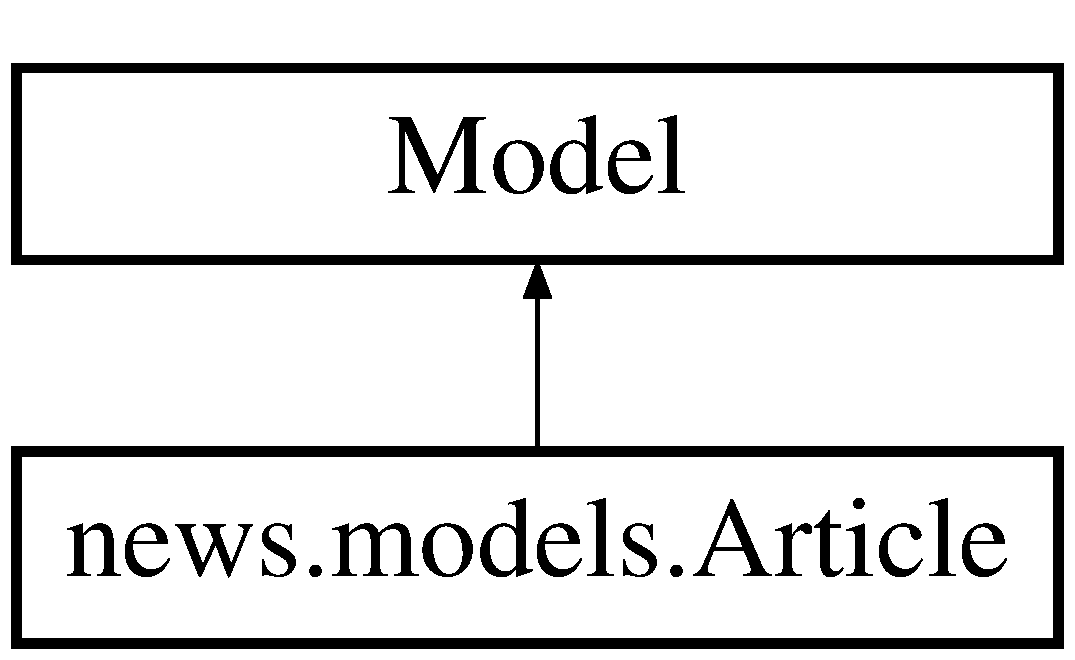
\includegraphics[height=2.000000cm]{classnews_1_1models_1_1_article}
\end{center}
\end{figure}
\subsection*{Static Public Attributes}
\begin{DoxyCompactItemize}
\item 
\mbox{\hyperlink{classnews_1_1models_1_1_article_a842d0d512e3991f1a5311205efe4fae9}{title}} = models.\+Char\+Field(max\+\_\+length=100, verbose\+\_\+name=\+\_\+(\textquotesingle{}Title\textquotesingle{}))
\end{DoxyCompactItemize}


\subsection{Detailed Description}
\begin{DoxyVerb}Documentation for a class.
\end{DoxyVerb}
 

\subsection{Member Data Documentation}
\mbox{\Hypertarget{classnews_1_1models_1_1_article_a842d0d512e3991f1a5311205efe4fae9}\label{classnews_1_1models_1_1_article_a842d0d512e3991f1a5311205efe4fae9}} 
\index{news\+::models\+::\+Article@{news\+::models\+::\+Article}!title@{title}}
\index{title@{title}!news\+::models\+::\+Article@{news\+::models\+::\+Article}}
\subsubsection{\texorpdfstring{title}{title}}
{\footnotesize\ttfamily news.\+models.\+Article.\+title = models.\+Char\+Field(max\+\_\+length=100, verbose\+\_\+name=\+\_\+(\textquotesingle{}Title\textquotesingle{}))\hspace{0.3cm}{\ttfamily [static]}}



The documentation for this class was generated from the following file\+:\begin{DoxyCompactItemize}
\item 
news/\mbox{\hyperlink{models_8py}{models.\+py}}\end{DoxyCompactItemize}

\hypertarget{classnews_1_1translation_1_1_article_translation_options}{}\section{news.\+translation.\+Article\+Translation\+Options Class Reference}
\label{classnews_1_1translation_1_1_article_translation_options}\index{news.\+translation.\+Article\+Translation\+Options@{news.\+translation.\+Article\+Translation\+Options}}
Inheritance diagram for news.\+translation.\+Article\+Translation\+Options\+:\begin{figure}[H]
\begin{center}
\leavevmode
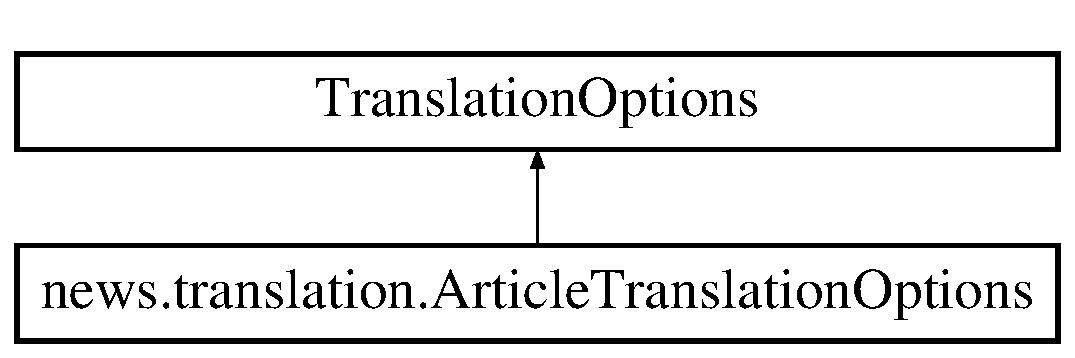
\includegraphics[height=2.000000cm]{classnews_1_1translation_1_1_article_translation_options}
\end{center}
\end{figure}
\subsection*{Static Public Attributes}
\begin{DoxyCompactItemize}
\item 
tuple \mbox{\hyperlink{classnews_1_1translation_1_1_article_translation_options_abda1e033b96cad8a40f2ccb6f5c7cc42}{fields}} = (\textquotesingle{}title\textquotesingle{},)
\end{DoxyCompactItemize}


\subsection{Member Data Documentation}
\mbox{\Hypertarget{classnews_1_1translation_1_1_article_translation_options_abda1e033b96cad8a40f2ccb6f5c7cc42}\label{classnews_1_1translation_1_1_article_translation_options_abda1e033b96cad8a40f2ccb6f5c7cc42}} 
\index{news\+::translation\+::\+Article\+Translation\+Options@{news\+::translation\+::\+Article\+Translation\+Options}!fields@{fields}}
\index{fields@{fields}!news\+::translation\+::\+Article\+Translation\+Options@{news\+::translation\+::\+Article\+Translation\+Options}}
\subsubsection{\texorpdfstring{fields}{fields}}
{\footnotesize\ttfamily tuple news.\+translation.\+Article\+Translation\+Options.\+fields = (\textquotesingle{}title\textquotesingle{},)\hspace{0.3cm}{\ttfamily [static]}}



The documentation for this class was generated from the following file\+:\begin{DoxyCompactItemize}
\item 
news/\mbox{\hyperlink{translation_8py}{translation.\+py}}\end{DoxyCompactItemize}

\hypertarget{classnews_1_1models_1_1_blog}{}\section{news.\+models.\+Blog Class Reference}
\label{classnews_1_1models_1_1_blog}\index{news.\+models.\+Blog@{news.\+models.\+Blog}}
Inheritance diagram for news.\+models.\+Blog\+:\begin{figure}[H]
\begin{center}
\leavevmode
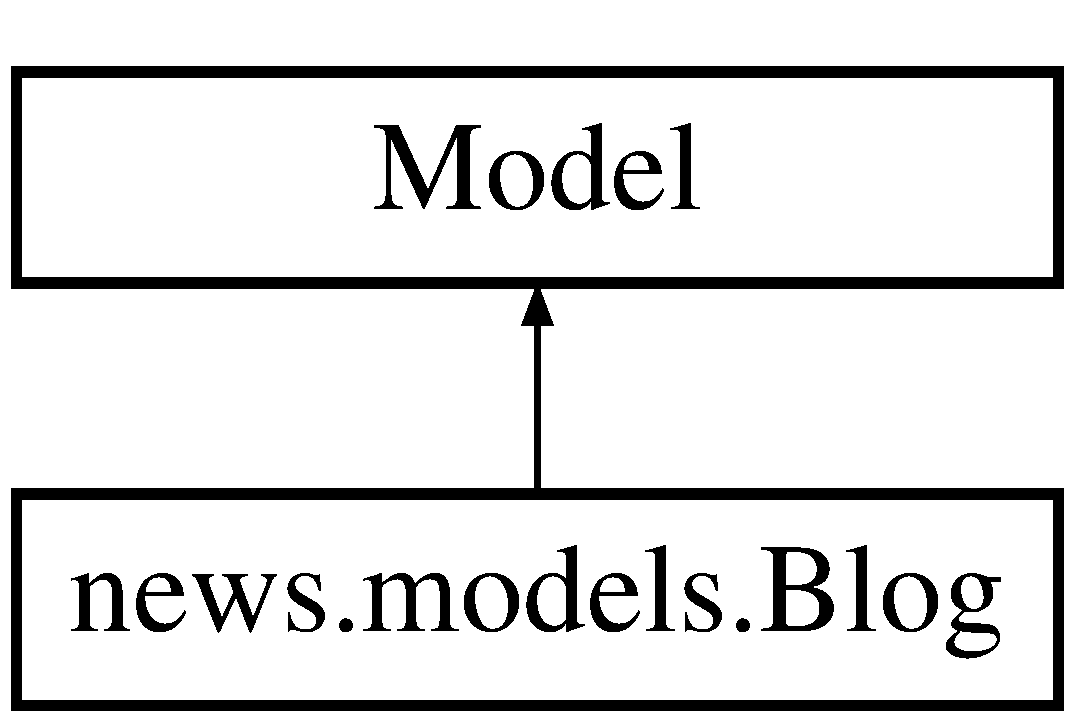
\includegraphics[height=2.000000cm]{classnews_1_1models_1_1_blog}
\end{center}
\end{figure}
\subsection*{Public Member Functions}
\begin{DoxyCompactItemize}
\item 
def \mbox{\hyperlink{classnews_1_1models_1_1_blog_a5cf49bbf405b3dfcbbe79905827ee3e7}{\+\_\+\+\_\+str\+\_\+\+\_\+}} (self)
\begin{DoxyCompactList}\small\item\em Documentation for a function. \end{DoxyCompactList}\end{DoxyCompactItemize}
\subsection*{Static Public Attributes}
\begin{DoxyCompactItemize}
\item 
\mbox{\hyperlink{classnews_1_1models_1_1_blog_a0ce1740083f2e95fa0d6709b795a2be3}{section}} = models.\+Char\+Field(max\+\_\+length=20)
\item 
\mbox{\hyperlink{classnews_1_1models_1_1_blog_a6adf7861b13c6898f5b74d18e91bf8c7}{title}} = models.\+Char\+Field(max\+\_\+length=50)
\item 
\mbox{\hyperlink{classnews_1_1models_1_1_blog_a44b6e01f0f7ca6ae9bd23477755efc81}{rating}} = models.\+Integer\+Field()
\item 
\mbox{\hyperlink{classnews_1_1models_1_1_blog_aee461adb8edec4537b75b01175074aba}{text}} = models.\+Char\+Field(max\+\_\+length=100)
\end{DoxyCompactItemize}


\subsection{Detailed Description}
\begin{DoxyVerb}    @brief Краткое описание

    Полное описание

    Attributes:
        id: achievement identifier
        type: type of achievement
        n: amount of elementary actions enough to get achievement\end{DoxyVerb}
 

\subsection{Member Function Documentation}
\mbox{\Hypertarget{classnews_1_1models_1_1_blog_a5cf49bbf405b3dfcbbe79905827ee3e7}\label{classnews_1_1models_1_1_blog_a5cf49bbf405b3dfcbbe79905827ee3e7}} 
\index{news\+::models\+::\+Blog@{news\+::models\+::\+Blog}!\+\_\+\+\_\+str\+\_\+\+\_\+@{\+\_\+\+\_\+str\+\_\+\+\_\+}}
\index{\+\_\+\+\_\+str\+\_\+\+\_\+@{\+\_\+\+\_\+str\+\_\+\+\_\+}!news\+::models\+::\+Blog@{news\+::models\+::\+Blog}}
\subsubsection{\texorpdfstring{\+\_\+\+\_\+str\+\_\+\+\_\+()}{\_\_str\_\_()}}
{\footnotesize\ttfamily def news.\+models.\+Blog.\+\_\+\+\_\+str\+\_\+\+\_\+ (\begin{DoxyParamCaption}\item[{}]{self }\end{DoxyParamCaption})}



Documentation for a function. 

Данная функция реализует алгоритм Евклида, при помощи которого находится наибольшее общее кратное у двух чисел.

\begin{DoxyAuthor}{Author}
Igor 
\end{DoxyAuthor}
\begin{DoxyWarning}{Warning}
Необходимо тестирование 
\end{DoxyWarning}
\begin{DoxyRefDesc}{Bug}
\item[\mbox{\hyperlink{bug__bug000001}{Bug}}]Описание бага \end{DoxyRefDesc}
\begin{DoxyVersion}{Version}
1.\+0 
\end{DoxyVersion}
\begin{DoxyDate}{Date}
14.\+10.\+2018 
\end{DoxyDate}
\begin{DoxyPrecond}{Precondition}
Предварительное условие 
\end{DoxyPrecond}
\begin{DoxyRefDesc}{Todo}
\item[\mbox{\hyperlink{todo__todo000001}{Todo}}]Дописать пару функций 

Протестить\end{DoxyRefDesc}



\begin{DoxyParams}{Parameters}
{\em a} & Параметр 1 \\
\hline
{\em b} & Параметр 2 \\
\hline
\end{DoxyParams}
\begin{DoxyReturn}{Returns}
Сумму двух чисел, переданных в качестве аргументов
\end{DoxyReturn}
Код функции выглядит следующим образом\+: 
\begin{DoxyCode}
    int gcd(int a, int b) \{
int r;
\textcolor{keywordflow}{while} (b) \{
    r = a % b;
    a = b;
    b = r;
\}
\textcolor{keywordflow}{return} r;
    \}
\end{DoxyCode}
 

\subsection{Member Data Documentation}
\mbox{\Hypertarget{classnews_1_1models_1_1_blog_a44b6e01f0f7ca6ae9bd23477755efc81}\label{classnews_1_1models_1_1_blog_a44b6e01f0f7ca6ae9bd23477755efc81}} 
\index{news\+::models\+::\+Blog@{news\+::models\+::\+Blog}!rating@{rating}}
\index{rating@{rating}!news\+::models\+::\+Blog@{news\+::models\+::\+Blog}}
\subsubsection{\texorpdfstring{rating}{rating}}
{\footnotesize\ttfamily news.\+models.\+Blog.\+rating = models.\+Integer\+Field()\hspace{0.3cm}{\ttfamily [static]}}

\mbox{\Hypertarget{classnews_1_1models_1_1_blog_a0ce1740083f2e95fa0d6709b795a2be3}\label{classnews_1_1models_1_1_blog_a0ce1740083f2e95fa0d6709b795a2be3}} 
\index{news\+::models\+::\+Blog@{news\+::models\+::\+Blog}!section@{section}}
\index{section@{section}!news\+::models\+::\+Blog@{news\+::models\+::\+Blog}}
\subsubsection{\texorpdfstring{section}{section}}
{\footnotesize\ttfamily news.\+models.\+Blog.\+section = models.\+Char\+Field(max\+\_\+length=20)\hspace{0.3cm}{\ttfamily [static]}}

\mbox{\Hypertarget{classnews_1_1models_1_1_blog_aee461adb8edec4537b75b01175074aba}\label{classnews_1_1models_1_1_blog_aee461adb8edec4537b75b01175074aba}} 
\index{news\+::models\+::\+Blog@{news\+::models\+::\+Blog}!text@{text}}
\index{text@{text}!news\+::models\+::\+Blog@{news\+::models\+::\+Blog}}
\subsubsection{\texorpdfstring{text}{text}}
{\footnotesize\ttfamily news.\+models.\+Blog.\+text = models.\+Char\+Field(max\+\_\+length=100)\hspace{0.3cm}{\ttfamily [static]}}

\mbox{\Hypertarget{classnews_1_1models_1_1_blog_a6adf7861b13c6898f5b74d18e91bf8c7}\label{classnews_1_1models_1_1_blog_a6adf7861b13c6898f5b74d18e91bf8c7}} 
\index{news\+::models\+::\+Blog@{news\+::models\+::\+Blog}!title@{title}}
\index{title@{title}!news\+::models\+::\+Blog@{news\+::models\+::\+Blog}}
\subsubsection{\texorpdfstring{title}{title}}
{\footnotesize\ttfamily news.\+models.\+Blog.\+title = models.\+Char\+Field(max\+\_\+length=50)\hspace{0.3cm}{\ttfamily [static]}}



The documentation for this class was generated from the following file\+:\begin{DoxyCompactItemize}
\item 
news/\mbox{\hyperlink{models_8py}{models.\+py}}\end{DoxyCompactItemize}

\hypertarget{classnews_1_1admin_1_1_blog_admin}{}\section{news.\+admin.\+Blog\+Admin Class Reference}
\label{classnews_1_1admin_1_1_blog_admin}\index{news.\+admin.\+Blog\+Admin@{news.\+admin.\+Blog\+Admin}}
Inheritance diagram for news.\+admin.\+Blog\+Admin\+:\begin{figure}[H]
\begin{center}
\leavevmode
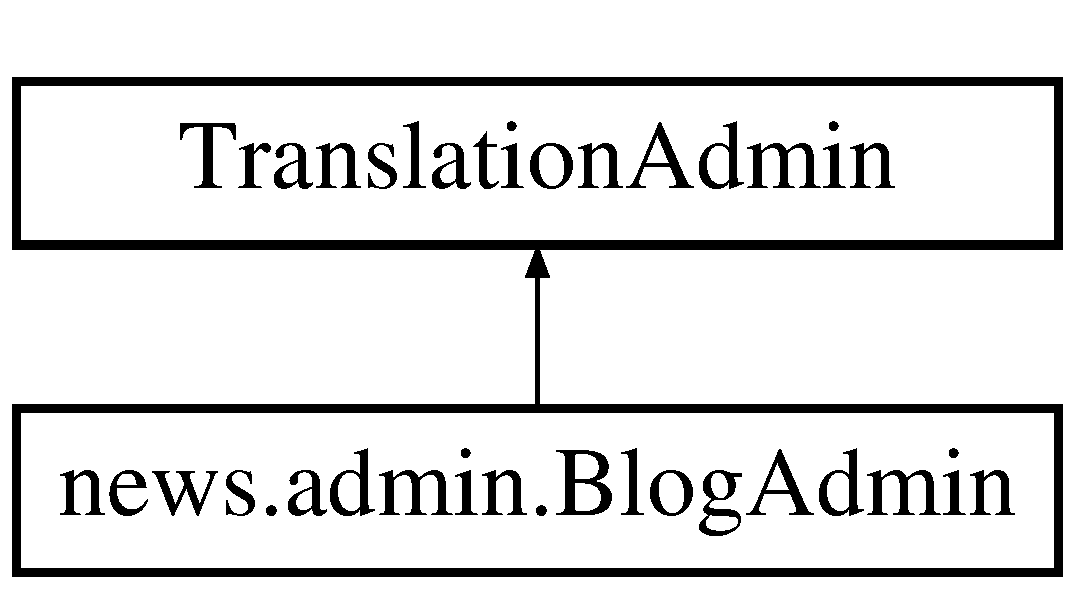
\includegraphics[height=2.000000cm]{classnews_1_1admin_1_1_blog_admin}
\end{center}
\end{figure}


The documentation for this class was generated from the following file\+:\begin{DoxyCompactItemize}
\item 
news/\mbox{\hyperlink{admin_8py}{admin.\+py}}\end{DoxyCompactItemize}

\hypertarget{classnews_1_1serializers_1_1_blog_serializer}{}\section{news.\+serializers.\+Blog\+Serializer Class Reference}
\label{classnews_1_1serializers_1_1_blog_serializer}\index{news.\+serializers.\+Blog\+Serializer@{news.\+serializers.\+Blog\+Serializer}}
Inheritance diagram for news.\+serializers.\+Blog\+Serializer\+:\begin{figure}[H]
\begin{center}
\leavevmode
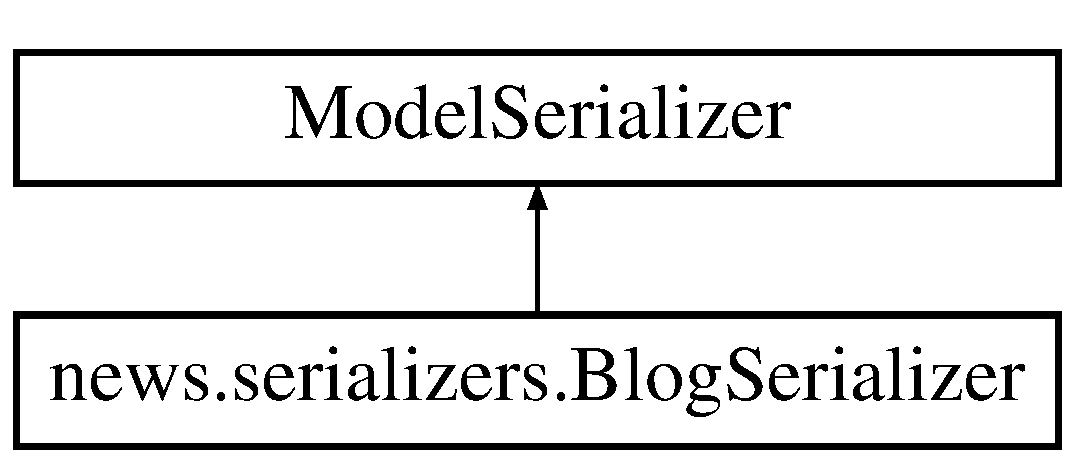
\includegraphics[height=2.000000cm]{classnews_1_1serializers_1_1_blog_serializer}
\end{center}
\end{figure}
\subsection*{Classes}
\begin{DoxyCompactItemize}
\item 
class \mbox{\hyperlink{classnews_1_1serializers_1_1_blog_serializer_1_1_meta}{Meta}}
\end{DoxyCompactItemize}


The documentation for this class was generated from the following file\+:\begin{DoxyCompactItemize}
\item 
news/\mbox{\hyperlink{serializers_8py}{serializers.\+py}}\end{DoxyCompactItemize}

\hypertarget{classnews_1_1translation_1_1_blog_translation_options}{}\section{news.\+translation.\+Blog\+Translation\+Options Class Reference}
\label{classnews_1_1translation_1_1_blog_translation_options}\index{news.\+translation.\+Blog\+Translation\+Options@{news.\+translation.\+Blog\+Translation\+Options}}
Inheritance diagram for news.\+translation.\+Blog\+Translation\+Options\+:\begin{figure}[H]
\begin{center}
\leavevmode
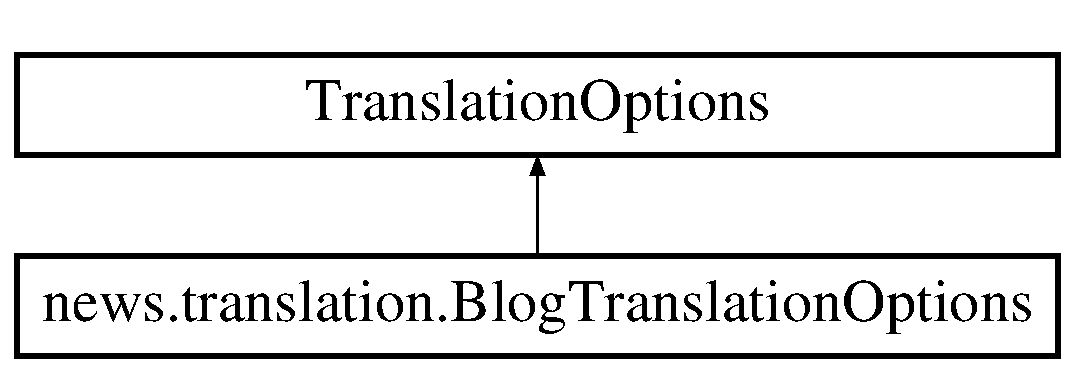
\includegraphics[height=2.000000cm]{classnews_1_1translation_1_1_blog_translation_options}
\end{center}
\end{figure}
\subsection*{Static Public Attributes}
\begin{DoxyCompactItemize}
\item 
tuple \mbox{\hyperlink{classnews_1_1translation_1_1_blog_translation_options_abc5be6b7080eafd09766bfa7096c4c7f}{fields}} = (\textquotesingle{}section\textquotesingle{}, \textquotesingle{}title\textquotesingle{}, \textquotesingle{}text\textquotesingle{})
\end{DoxyCompactItemize}


\subsection{Member Data Documentation}
\mbox{\Hypertarget{classnews_1_1translation_1_1_blog_translation_options_abc5be6b7080eafd09766bfa7096c4c7f}\label{classnews_1_1translation_1_1_blog_translation_options_abc5be6b7080eafd09766bfa7096c4c7f}} 
\index{news\+::translation\+::\+Blog\+Translation\+Options@{news\+::translation\+::\+Blog\+Translation\+Options}!fields@{fields}}
\index{fields@{fields}!news\+::translation\+::\+Blog\+Translation\+Options@{news\+::translation\+::\+Blog\+Translation\+Options}}
\subsubsection{\texorpdfstring{fields}{fields}}
{\footnotesize\ttfamily tuple news.\+translation.\+Blog\+Translation\+Options.\+fields = (\textquotesingle{}section\textquotesingle{}, \textquotesingle{}title\textquotesingle{}, \textquotesingle{}text\textquotesingle{})\hspace{0.3cm}{\ttfamily [static]}}



The documentation for this class was generated from the following file\+:\begin{DoxyCompactItemize}
\item 
news/\mbox{\hyperlink{translation_8py}{translation.\+py}}\end{DoxyCompactItemize}

\hypertarget{classnews_1_1views_1_1_blog_view_set}{}\section{news.\+views.\+Blog\+View\+Set Class Reference}
\label{classnews_1_1views_1_1_blog_view_set}\index{news.\+views.\+Blog\+View\+Set@{news.\+views.\+Blog\+View\+Set}}
Inheritance diagram for news.\+views.\+Blog\+View\+Set\+:\begin{figure}[H]
\begin{center}
\leavevmode
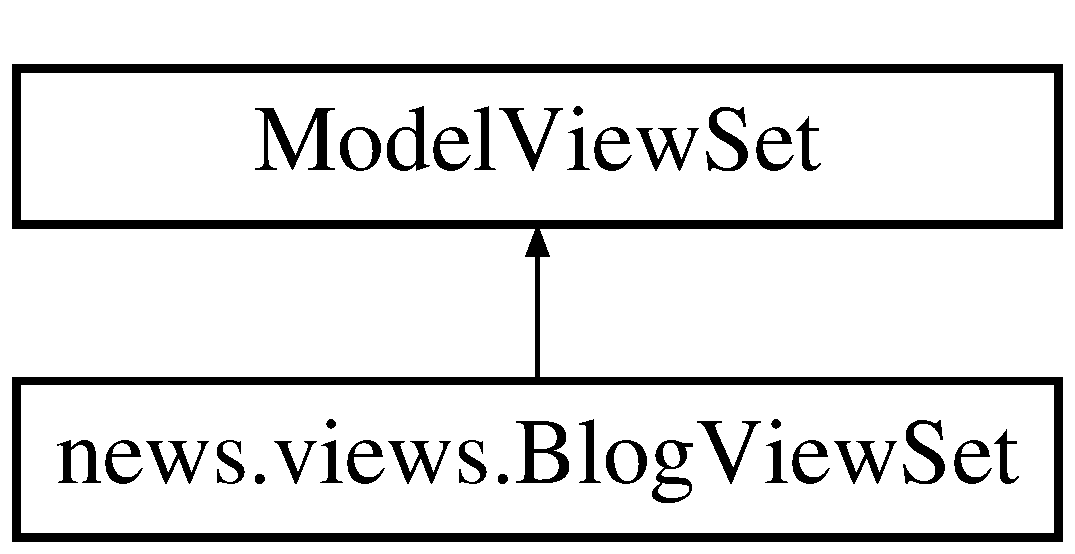
\includegraphics[height=2.000000cm]{classnews_1_1views_1_1_blog_view_set}
\end{center}
\end{figure}
\subsection*{Static Public Attributes}
\begin{DoxyCompactItemize}
\item 
\mbox{\hyperlink{classnews_1_1views_1_1_blog_view_set_a1ebd2b9347e2c0bc632416288d723219}{queryset}} = Blog.\+objects.\+all()
\item 
\mbox{\hyperlink{classnews_1_1views_1_1_blog_view_set_aa2cb1ca862d1df2069cea4bb061cf1ba}{serializer\+\_\+class}} = \mbox{\hyperlink{classnews_1_1serializers_1_1_blog_serializer}{Blog\+Serializer}}
\end{DoxyCompactItemize}


\subsection{Member Data Documentation}
\mbox{\Hypertarget{classnews_1_1views_1_1_blog_view_set_a1ebd2b9347e2c0bc632416288d723219}\label{classnews_1_1views_1_1_blog_view_set_a1ebd2b9347e2c0bc632416288d723219}} 
\index{news\+::views\+::\+Blog\+View\+Set@{news\+::views\+::\+Blog\+View\+Set}!queryset@{queryset}}
\index{queryset@{queryset}!news\+::views\+::\+Blog\+View\+Set@{news\+::views\+::\+Blog\+View\+Set}}
\subsubsection{\texorpdfstring{queryset}{queryset}}
{\footnotesize\ttfamily news.\+views.\+Blog\+View\+Set.\+queryset = Blog.\+objects.\+all()\hspace{0.3cm}{\ttfamily [static]}}

\mbox{\Hypertarget{classnews_1_1views_1_1_blog_view_set_aa2cb1ca862d1df2069cea4bb061cf1ba}\label{classnews_1_1views_1_1_blog_view_set_aa2cb1ca862d1df2069cea4bb061cf1ba}} 
\index{news\+::views\+::\+Blog\+View\+Set@{news\+::views\+::\+Blog\+View\+Set}!serializer\+\_\+class@{serializer\+\_\+class}}
\index{serializer\+\_\+class@{serializer\+\_\+class}!news\+::views\+::\+Blog\+View\+Set@{news\+::views\+::\+Blog\+View\+Set}}
\subsubsection{\texorpdfstring{serializer\+\_\+class}{serializer\_class}}
{\footnotesize\ttfamily news.\+views.\+Blog\+View\+Set.\+serializer\+\_\+class = \mbox{\hyperlink{classnews_1_1serializers_1_1_blog_serializer}{Blog\+Serializer}}\hspace{0.3cm}{\ttfamily [static]}}



The documentation for this class was generated from the following file\+:\begin{DoxyCompactItemize}
\item 
news/\mbox{\hyperlink{views_8py}{views.\+py}}\end{DoxyCompactItemize}

\hypertarget{classnews_1_1serializers_1_1_blog_serializer_1_1_meta}{}\section{news.\+serializers.\+Blog\+Serializer.\+Meta Class Reference}
\label{classnews_1_1serializers_1_1_blog_serializer_1_1_meta}\index{news.\+serializers.\+Blog\+Serializer.\+Meta@{news.\+serializers.\+Blog\+Serializer.\+Meta}}
\subsection*{Static Public Attributes}
\begin{DoxyCompactItemize}
\item 
\mbox{\hyperlink{classnews_1_1serializers_1_1_blog_serializer_1_1_meta_ab2a309acb0e3758709b853f234dc3f0d}{model}} = \mbox{\hyperlink{classnews_1_1models_1_1_blog}{Blog}}
\item 
tuple \mbox{\hyperlink{classnews_1_1serializers_1_1_blog_serializer_1_1_meta_a0268bed058b50064615f2e10b04f2571}{fields}} = (\textquotesingle{}section\textquotesingle{}, \textquotesingle{}title\textquotesingle{}, \textquotesingle{}rating\textquotesingle{}, \textquotesingle{}text\textquotesingle{}, \textquotesingle{}title\+\_\+ru\textquotesingle{}, \textquotesingle{}title\+\_\+en\textquotesingle{}, \textquotesingle{}title\+\_\+de\textquotesingle{})
\end{DoxyCompactItemize}


\subsection{Member Data Documentation}
\mbox{\Hypertarget{classnews_1_1serializers_1_1_blog_serializer_1_1_meta_a0268bed058b50064615f2e10b04f2571}\label{classnews_1_1serializers_1_1_blog_serializer_1_1_meta_a0268bed058b50064615f2e10b04f2571}} 
\index{news\+::serializers\+::\+Blog\+Serializer\+::\+Meta@{news\+::serializers\+::\+Blog\+Serializer\+::\+Meta}!fields@{fields}}
\index{fields@{fields}!news\+::serializers\+::\+Blog\+Serializer\+::\+Meta@{news\+::serializers\+::\+Blog\+Serializer\+::\+Meta}}
\subsubsection{\texorpdfstring{fields}{fields}}
{\footnotesize\ttfamily tuple news.\+serializers.\+Blog\+Serializer.\+Meta.\+fields = (\textquotesingle{}section\textquotesingle{}, \textquotesingle{}title\textquotesingle{}, \textquotesingle{}rating\textquotesingle{}, \textquotesingle{}text\textquotesingle{}, \textquotesingle{}title\+\_\+ru\textquotesingle{}, \textquotesingle{}title\+\_\+en\textquotesingle{}, \textquotesingle{}title\+\_\+de\textquotesingle{})\hspace{0.3cm}{\ttfamily [static]}}

\mbox{\Hypertarget{classnews_1_1serializers_1_1_blog_serializer_1_1_meta_ab2a309acb0e3758709b853f234dc3f0d}\label{classnews_1_1serializers_1_1_blog_serializer_1_1_meta_ab2a309acb0e3758709b853f234dc3f0d}} 
\index{news\+::serializers\+::\+Blog\+Serializer\+::\+Meta@{news\+::serializers\+::\+Blog\+Serializer\+::\+Meta}!model@{model}}
\index{model@{model}!news\+::serializers\+::\+Blog\+Serializer\+::\+Meta@{news\+::serializers\+::\+Blog\+Serializer\+::\+Meta}}
\subsubsection{\texorpdfstring{model}{model}}
{\footnotesize\ttfamily news.\+serializers.\+Blog\+Serializer.\+Meta.\+model = \mbox{\hyperlink{classnews_1_1models_1_1_blog}{Blog}}\hspace{0.3cm}{\ttfamily [static]}}



The documentation for this class was generated from the following file\+:\begin{DoxyCompactItemize}
\item 
news/\mbox{\hyperlink{serializers_8py}{serializers.\+py}}\end{DoxyCompactItemize}

\hypertarget{classnews_1_1migrations_1_10004__delete__text_1_1_migration}{}\section{news.\+migrations.0004\+\_\+delete\+\_\+text.Migration Class Reference}
\label{classnews_1_1migrations_1_10004__delete__text_1_1_migration}\index{news.\+migrations.\+0004\+\_\+delete\+\_\+text.\+Migration@{news.\+migrations.\+0004\+\_\+delete\+\_\+text.\+Migration}}
Inheritance diagram for news.\+migrations.0004\+\_\+delete\+\_\+text.Migration\+:\begin{figure}[H]
\begin{center}
\leavevmode
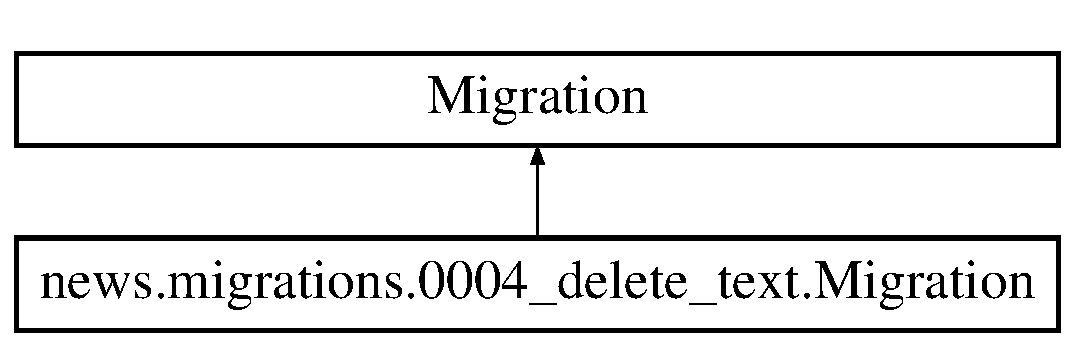
\includegraphics[height=2.000000cm]{classnews_1_1migrations_1_10004__delete__text_1_1_migration}
\end{center}
\end{figure}
\subsection*{Static Public Attributes}
\begin{DoxyCompactItemize}
\item 
list \mbox{\hyperlink{classnews_1_1migrations_1_10004__delete__text_1_1_migration_a8ffd54d8b8a09e031987f159e869208f}{dependencies}}
\item 
list \mbox{\hyperlink{classnews_1_1migrations_1_10004__delete__text_1_1_migration_a2f379b87d68991adbc82291d97785652}{operations}}
\end{DoxyCompactItemize}


\subsection{Member Data Documentation}
\mbox{\Hypertarget{classnews_1_1migrations_1_10004__delete__text_1_1_migration_a8ffd54d8b8a09e031987f159e869208f}\label{classnews_1_1migrations_1_10004__delete__text_1_1_migration_a8ffd54d8b8a09e031987f159e869208f}} 
\index{news\+::migrations\+::0004\+\_\+delete\+\_\+text\+::\+Migration@{news\+::migrations\+::0004\+\_\+delete\+\_\+text\+::\+Migration}!dependencies@{dependencies}}
\index{dependencies@{dependencies}!news\+::migrations\+::0004\+\_\+delete\+\_\+text\+::\+Migration@{news\+::migrations\+::0004\+\_\+delete\+\_\+text\+::\+Migration}}
\subsubsection{\texorpdfstring{dependencies}{dependencies}}
{\footnotesize\ttfamily list news.\+migrations.\+0004\+\_\+delete\+\_\+text.\+Migration.\+dependencies\hspace{0.3cm}{\ttfamily [static]}}

{\bfseries Initial value\+:}
\begin{DoxyCode}
=  [
        (\textcolor{stringliteral}{'news'}, \textcolor{stringliteral}{'0003\_text'}),
    ]
\end{DoxyCode}
\mbox{\Hypertarget{classnews_1_1migrations_1_10004__delete__text_1_1_migration_a2f379b87d68991adbc82291d97785652}\label{classnews_1_1migrations_1_10004__delete__text_1_1_migration_a2f379b87d68991adbc82291d97785652}} 
\index{news\+::migrations\+::0004\+\_\+delete\+\_\+text\+::\+Migration@{news\+::migrations\+::0004\+\_\+delete\+\_\+text\+::\+Migration}!operations@{operations}}
\index{operations@{operations}!news\+::migrations\+::0004\+\_\+delete\+\_\+text\+::\+Migration@{news\+::migrations\+::0004\+\_\+delete\+\_\+text\+::\+Migration}}
\subsubsection{\texorpdfstring{operations}{operations}}
{\footnotesize\ttfamily list news.\+migrations.\+0004\+\_\+delete\+\_\+text.\+Migration.\+operations\hspace{0.3cm}{\ttfamily [static]}}

{\bfseries Initial value\+:}
\begin{DoxyCode}
=  [
        migrations.DeleteModel(
            name=\textcolor{stringliteral}{'Text'},
        ),
    ]
\end{DoxyCode}


The documentation for this class was generated from the following file\+:\begin{DoxyCompactItemize}
\item 
news/migrations/\mbox{\hyperlink{0004__delete__text_8py}{0004\+\_\+delete\+\_\+text.\+py}}\end{DoxyCompactItemize}

\hypertarget{classnews_1_1migrations_1_10005__blog_1_1_migration}{}\section{news.\+migrations.0005\+\_\+blog.Migration Class Reference}
\label{classnews_1_1migrations_1_10005__blog_1_1_migration}\index{news.\+migrations.\+0005\+\_\+blog.\+Migration@{news.\+migrations.\+0005\+\_\+blog.\+Migration}}
Inheritance diagram for news.\+migrations.0005\+\_\+blog.Migration\+:\begin{figure}[H]
\begin{center}
\leavevmode
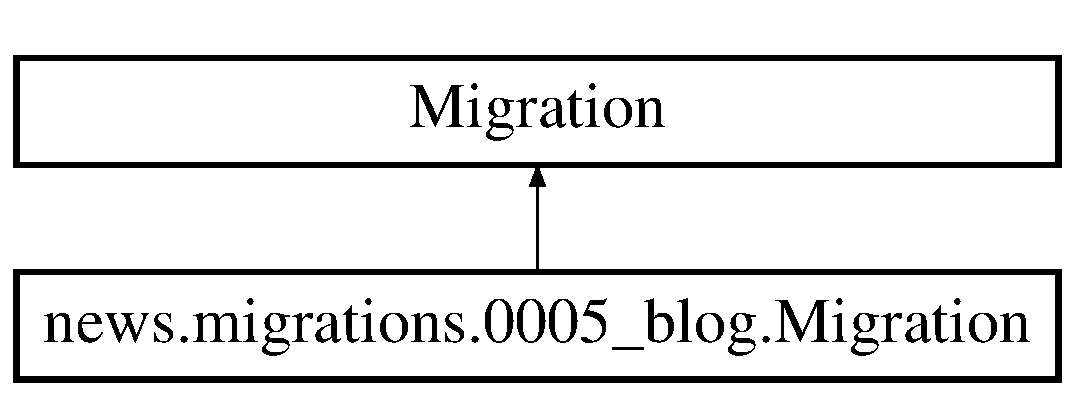
\includegraphics[height=2.000000cm]{classnews_1_1migrations_1_10005__blog_1_1_migration}
\end{center}
\end{figure}
\subsection*{Static Public Attributes}
\begin{DoxyCompactItemize}
\item 
list \mbox{\hyperlink{classnews_1_1migrations_1_10005__blog_1_1_migration_a67fe13fe5bba063eb0b2f6814e84dd44}{dependencies}}
\item 
list \mbox{\hyperlink{classnews_1_1migrations_1_10005__blog_1_1_migration_ac1237edc72e8630319b2134ee14c3305}{operations}}
\end{DoxyCompactItemize}


\subsection{Member Data Documentation}
\mbox{\Hypertarget{classnews_1_1migrations_1_10005__blog_1_1_migration_a67fe13fe5bba063eb0b2f6814e84dd44}\label{classnews_1_1migrations_1_10005__blog_1_1_migration_a67fe13fe5bba063eb0b2f6814e84dd44}} 
\index{news\+::migrations\+::0005\+\_\+blog\+::\+Migration@{news\+::migrations\+::0005\+\_\+blog\+::\+Migration}!dependencies@{dependencies}}
\index{dependencies@{dependencies}!news\+::migrations\+::0005\+\_\+blog\+::\+Migration@{news\+::migrations\+::0005\+\_\+blog\+::\+Migration}}
\subsubsection{\texorpdfstring{dependencies}{dependencies}}
{\footnotesize\ttfamily list news.\+migrations.\+0005\+\_\+blog.\+Migration.\+dependencies\hspace{0.3cm}{\ttfamily [static]}}

{\bfseries Initial value\+:}
\begin{DoxyCode}
=  [
        (\textcolor{stringliteral}{'news'}, \textcolor{stringliteral}{'0004\_delete\_text'}),
    ]
\end{DoxyCode}
\mbox{\Hypertarget{classnews_1_1migrations_1_10005__blog_1_1_migration_ac1237edc72e8630319b2134ee14c3305}\label{classnews_1_1migrations_1_10005__blog_1_1_migration_ac1237edc72e8630319b2134ee14c3305}} 
\index{news\+::migrations\+::0005\+\_\+blog\+::\+Migration@{news\+::migrations\+::0005\+\_\+blog\+::\+Migration}!operations@{operations}}
\index{operations@{operations}!news\+::migrations\+::0005\+\_\+blog\+::\+Migration@{news\+::migrations\+::0005\+\_\+blog\+::\+Migration}}
\subsubsection{\texorpdfstring{operations}{operations}}
{\footnotesize\ttfamily list news.\+migrations.\+0005\+\_\+blog.\+Migration.\+operations\hspace{0.3cm}{\ttfamily [static]}}

{\bfseries Initial value\+:}
\begin{DoxyCode}
=  [
        migrations.CreateModel(
            name=\textcolor{stringliteral}{'Blog'},
            fields=[
                (\textcolor{stringliteral}{'id'}, models.AutoField(auto\_created=\textcolor{keyword}{True}, primary\_key=\textcolor{keyword}{True}, serialize=\textcolor{keyword}{False}, verbose\_name=\textcolor{stringliteral}{
      'ID'})),
                (\textcolor{stringliteral}{'section'}, models.CharField(max\_length=20)),
                (\textcolor{stringliteral}{'title'}, models.CharField(max\_length=50)),
                (\textcolor{stringliteral}{'rating'}, models.IntegerField()),
                (\textcolor{stringliteral}{'text'}, models.CharField(max\_length=100)),
            ],
        ),
    ]
\end{DoxyCode}


The documentation for this class was generated from the following file\+:\begin{DoxyCompactItemize}
\item 
news/migrations/\mbox{\hyperlink{0005__blog_8py}{0005\+\_\+blog.\+py}}\end{DoxyCompactItemize}

\hypertarget{classnews_1_1migrations_1_10006__auto__20181013__0120_1_1_migration}{}\section{news.\+migrations.0006\+\_\+auto\+\_\+20181013\+\_\+0120.Migration Class Reference}
\label{classnews_1_1migrations_1_10006__auto__20181013__0120_1_1_migration}\index{news.\+migrations.\+0006\+\_\+auto\+\_\+20181013\+\_\+0120.\+Migration@{news.\+migrations.\+0006\+\_\+auto\+\_\+20181013\+\_\+0120.\+Migration}}
Inheritance diagram for news.\+migrations.0006\+\_\+auto\+\_\+20181013\+\_\+0120.Migration\+:\begin{figure}[H]
\begin{center}
\leavevmode
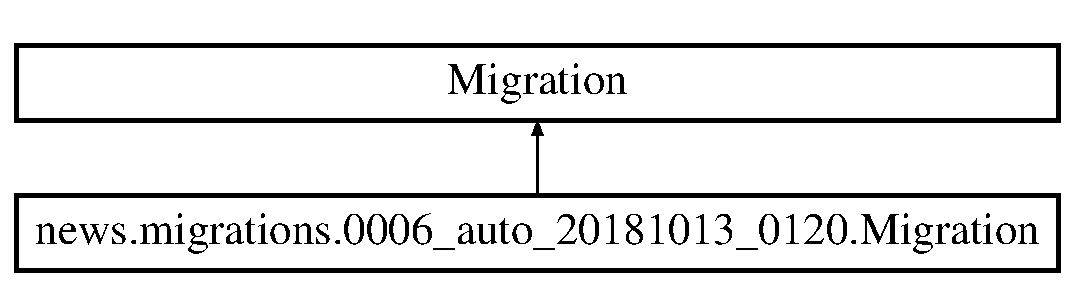
\includegraphics[height=2.000000cm]{classnews_1_1migrations_1_10006__auto__20181013__0120_1_1_migration}
\end{center}
\end{figure}
\subsection*{Static Public Attributes}
\begin{DoxyCompactItemize}
\item 
list \mbox{\hyperlink{classnews_1_1migrations_1_10006__auto__20181013__0120_1_1_migration_acfbb0610f371eec6715c603d63c5a0ac}{dependencies}}
\item 
list \mbox{\hyperlink{classnews_1_1migrations_1_10006__auto__20181013__0120_1_1_migration_a6c786bba5496eef9adf188f58419b94e}{operations}}
\end{DoxyCompactItemize}


\subsection{Member Data Documentation}
\mbox{\Hypertarget{classnews_1_1migrations_1_10006__auto__20181013__0120_1_1_migration_acfbb0610f371eec6715c603d63c5a0ac}\label{classnews_1_1migrations_1_10006__auto__20181013__0120_1_1_migration_acfbb0610f371eec6715c603d63c5a0ac}} 
\index{news\+::migrations\+::0006\+\_\+auto\+\_\+20181013\+\_\+0120\+::\+Migration@{news\+::migrations\+::0006\+\_\+auto\+\_\+20181013\+\_\+0120\+::\+Migration}!dependencies@{dependencies}}
\index{dependencies@{dependencies}!news\+::migrations\+::0006\+\_\+auto\+\_\+20181013\+\_\+0120\+::\+Migration@{news\+::migrations\+::0006\+\_\+auto\+\_\+20181013\+\_\+0120\+::\+Migration}}
\subsubsection{\texorpdfstring{dependencies}{dependencies}}
{\footnotesize\ttfamily list news.\+migrations.\+0006\+\_\+auto\+\_\+20181013\+\_\+0120.\+Migration.\+dependencies\hspace{0.3cm}{\ttfamily [static]}}

{\bfseries Initial value\+:}
\begin{DoxyCode}
=  [
        (\textcolor{stringliteral}{'news'}, \textcolor{stringliteral}{'0005\_blog'}),
    ]
\end{DoxyCode}
\mbox{\Hypertarget{classnews_1_1migrations_1_10006__auto__20181013__0120_1_1_migration_a6c786bba5496eef9adf188f58419b94e}\label{classnews_1_1migrations_1_10006__auto__20181013__0120_1_1_migration_a6c786bba5496eef9adf188f58419b94e}} 
\index{news\+::migrations\+::0006\+\_\+auto\+\_\+20181013\+\_\+0120\+::\+Migration@{news\+::migrations\+::0006\+\_\+auto\+\_\+20181013\+\_\+0120\+::\+Migration}!operations@{operations}}
\index{operations@{operations}!news\+::migrations\+::0006\+\_\+auto\+\_\+20181013\+\_\+0120\+::\+Migration@{news\+::migrations\+::0006\+\_\+auto\+\_\+20181013\+\_\+0120\+::\+Migration}}
\subsubsection{\texorpdfstring{operations}{operations}}
{\footnotesize\ttfamily list news.\+migrations.\+0006\+\_\+auto\+\_\+20181013\+\_\+0120.\+Migration.\+operations\hspace{0.3cm}{\ttfamily [static]}}



The documentation for this class was generated from the following file\+:\begin{DoxyCompactItemize}
\item 
news/migrations/\mbox{\hyperlink{0006__auto__20181013__0120_8py}{0006\+\_\+auto\+\_\+20181013\+\_\+0120.\+py}}\end{DoxyCompactItemize}

\hypertarget{classnews_1_1migrations_1_10002__auto__20181009__2006_1_1_migration}{}\section{news.\+migrations.0002\+\_\+auto\+\_\+20181009\+\_\+2006.Migration Class Reference}
\label{classnews_1_1migrations_1_10002__auto__20181009__2006_1_1_migration}\index{news.\+migrations.\+0002\+\_\+auto\+\_\+20181009\+\_\+2006.\+Migration@{news.\+migrations.\+0002\+\_\+auto\+\_\+20181009\+\_\+2006.\+Migration}}
Inheritance diagram for news.\+migrations.0002\+\_\+auto\+\_\+20181009\+\_\+2006.Migration\+:\begin{figure}[H]
\begin{center}
\leavevmode
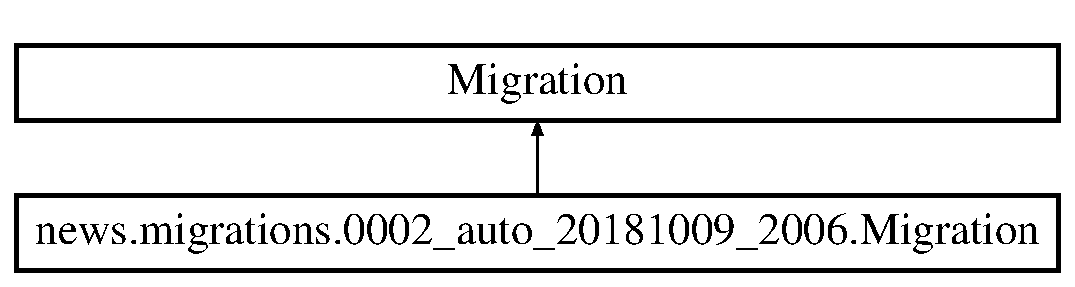
\includegraphics[height=2.000000cm]{classnews_1_1migrations_1_10002__auto__20181009__2006_1_1_migration}
\end{center}
\end{figure}
\subsection*{Static Public Attributes}
\begin{DoxyCompactItemize}
\item 
list \mbox{\hyperlink{classnews_1_1migrations_1_10002__auto__20181009__2006_1_1_migration_aa1978d83bfabe6b651534ac6ef626963}{dependencies}}
\item 
list \mbox{\hyperlink{classnews_1_1migrations_1_10002__auto__20181009__2006_1_1_migration_a243cfcb5672fe1a8555d980b0521dafa}{operations}}
\end{DoxyCompactItemize}


\subsection{Member Data Documentation}
\mbox{\Hypertarget{classnews_1_1migrations_1_10002__auto__20181009__2006_1_1_migration_aa1978d83bfabe6b651534ac6ef626963}\label{classnews_1_1migrations_1_10002__auto__20181009__2006_1_1_migration_aa1978d83bfabe6b651534ac6ef626963}} 
\index{news\+::migrations\+::0002\+\_\+auto\+\_\+20181009\+\_\+2006\+::\+Migration@{news\+::migrations\+::0002\+\_\+auto\+\_\+20181009\+\_\+2006\+::\+Migration}!dependencies@{dependencies}}
\index{dependencies@{dependencies}!news\+::migrations\+::0002\+\_\+auto\+\_\+20181009\+\_\+2006\+::\+Migration@{news\+::migrations\+::0002\+\_\+auto\+\_\+20181009\+\_\+2006\+::\+Migration}}
\subsubsection{\texorpdfstring{dependencies}{dependencies}}
{\footnotesize\ttfamily list news.\+migrations.\+0002\+\_\+auto\+\_\+20181009\+\_\+2006.\+Migration.\+dependencies\hspace{0.3cm}{\ttfamily [static]}}

{\bfseries Initial value\+:}
\begin{DoxyCode}
=  [
        (\textcolor{stringliteral}{'news'}, \textcolor{stringliteral}{'0001\_initial'}),
    ]
\end{DoxyCode}
\mbox{\Hypertarget{classnews_1_1migrations_1_10002__auto__20181009__2006_1_1_migration_a243cfcb5672fe1a8555d980b0521dafa}\label{classnews_1_1migrations_1_10002__auto__20181009__2006_1_1_migration_a243cfcb5672fe1a8555d980b0521dafa}} 
\index{news\+::migrations\+::0002\+\_\+auto\+\_\+20181009\+\_\+2006\+::\+Migration@{news\+::migrations\+::0002\+\_\+auto\+\_\+20181009\+\_\+2006\+::\+Migration}!operations@{operations}}
\index{operations@{operations}!news\+::migrations\+::0002\+\_\+auto\+\_\+20181009\+\_\+2006\+::\+Migration@{news\+::migrations\+::0002\+\_\+auto\+\_\+20181009\+\_\+2006\+::\+Migration}}
\subsubsection{\texorpdfstring{operations}{operations}}
{\footnotesize\ttfamily list news.\+migrations.\+0002\+\_\+auto\+\_\+20181009\+\_\+2006.\+Migration.\+operations\hspace{0.3cm}{\ttfamily [static]}}

{\bfseries Initial value\+:}
\begin{DoxyCode}
=  [
        migrations.AddField(
            model\_name=\textcolor{stringliteral}{'article'},
            name=\textcolor{stringliteral}{'title\_de'},
            field=models.CharField(max\_length=100, null=\textcolor{keyword}{True}, verbose\_name=\textcolor{stringliteral}{'Title'}),
        ),
        migrations.AddField(
            model\_name=\textcolor{stringliteral}{'article'},
            name=\textcolor{stringliteral}{'title\_en'},
            field=models.CharField(max\_length=100, null=\textcolor{keyword}{True}, verbose\_name=\textcolor{stringliteral}{'Title'}),
        ),
        migrations.AddField(
            model\_name=\textcolor{stringliteral}{'article'},
            name=\textcolor{stringliteral}{'title\_ru'},
            field=models.CharField(max\_length=100, null=\textcolor{keyword}{True}, verbose\_name=\textcolor{stringliteral}{'Title'}),
        ),
    ]
\end{DoxyCode}


The documentation for this class was generated from the following file\+:\begin{DoxyCompactItemize}
\item 
news/migrations/\mbox{\hyperlink{0002__auto__20181009__2006_8py}{0002\+\_\+auto\+\_\+20181009\+\_\+2006.\+py}}\end{DoxyCompactItemize}

\hypertarget{classnews_1_1migrations_1_10001__initial_1_1_migration}{}\section{news.\+migrations.0001\+\_\+initial.Migration Class Reference}
\label{classnews_1_1migrations_1_10001__initial_1_1_migration}\index{news.\+migrations.\+0001\+\_\+initial.\+Migration@{news.\+migrations.\+0001\+\_\+initial.\+Migration}}
Inheritance diagram for news.\+migrations.0001\+\_\+initial.Migration\+:\begin{figure}[H]
\begin{center}
\leavevmode
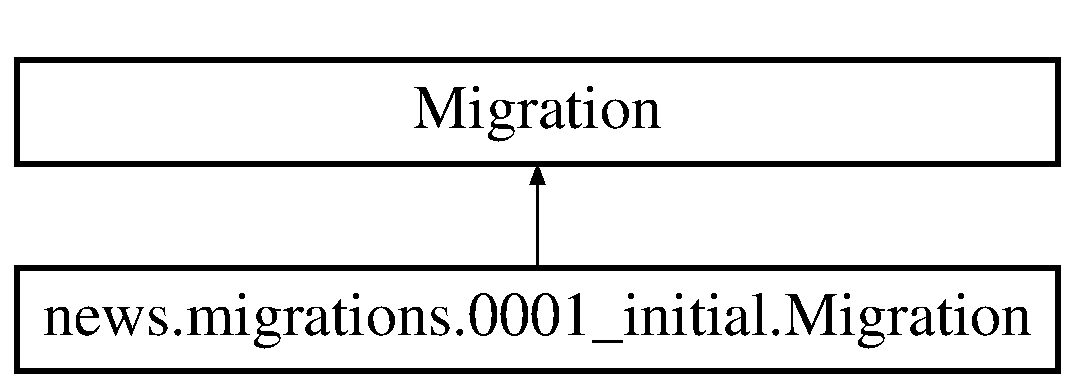
\includegraphics[height=2.000000cm]{classnews_1_1migrations_1_10001__initial_1_1_migration}
\end{center}
\end{figure}
\subsection*{Static Public Attributes}
\begin{DoxyCompactItemize}
\item 
bool \mbox{\hyperlink{classnews_1_1migrations_1_10001__initial_1_1_migration_aabc5dbf8fca555e21bb4e345893694a2}{initial}} = True
\item 
list \mbox{\hyperlink{classnews_1_1migrations_1_10001__initial_1_1_migration_a3fef00e0c6160b568045ee2b8f9e2684}{dependencies}}
\item 
list \mbox{\hyperlink{classnews_1_1migrations_1_10001__initial_1_1_migration_ae137eaa618a2a194cebaab9f59d42526}{operations}}
\end{DoxyCompactItemize}


\subsection{Member Data Documentation}
\mbox{\Hypertarget{classnews_1_1migrations_1_10001__initial_1_1_migration_a3fef00e0c6160b568045ee2b8f9e2684}\label{classnews_1_1migrations_1_10001__initial_1_1_migration_a3fef00e0c6160b568045ee2b8f9e2684}} 
\index{news\+::migrations\+::0001\+\_\+initial\+::\+Migration@{news\+::migrations\+::0001\+\_\+initial\+::\+Migration}!dependencies@{dependencies}}
\index{dependencies@{dependencies}!news\+::migrations\+::0001\+\_\+initial\+::\+Migration@{news\+::migrations\+::0001\+\_\+initial\+::\+Migration}}
\subsubsection{\texorpdfstring{dependencies}{dependencies}}
{\footnotesize\ttfamily list news.\+migrations.\+0001\+\_\+initial.\+Migration.\+dependencies\hspace{0.3cm}{\ttfamily [static]}}

{\bfseries Initial value\+:}
\begin{DoxyCode}
=  [
    ]
\end{DoxyCode}
\mbox{\Hypertarget{classnews_1_1migrations_1_10001__initial_1_1_migration_aabc5dbf8fca555e21bb4e345893694a2}\label{classnews_1_1migrations_1_10001__initial_1_1_migration_aabc5dbf8fca555e21bb4e345893694a2}} 
\index{news\+::migrations\+::0001\+\_\+initial\+::\+Migration@{news\+::migrations\+::0001\+\_\+initial\+::\+Migration}!initial@{initial}}
\index{initial@{initial}!news\+::migrations\+::0001\+\_\+initial\+::\+Migration@{news\+::migrations\+::0001\+\_\+initial\+::\+Migration}}
\subsubsection{\texorpdfstring{initial}{initial}}
{\footnotesize\ttfamily bool news.\+migrations.\+0001\+\_\+initial.\+Migration.\+initial = True\hspace{0.3cm}{\ttfamily [static]}}

\mbox{\Hypertarget{classnews_1_1migrations_1_10001__initial_1_1_migration_ae137eaa618a2a194cebaab9f59d42526}\label{classnews_1_1migrations_1_10001__initial_1_1_migration_ae137eaa618a2a194cebaab9f59d42526}} 
\index{news\+::migrations\+::0001\+\_\+initial\+::\+Migration@{news\+::migrations\+::0001\+\_\+initial\+::\+Migration}!operations@{operations}}
\index{operations@{operations}!news\+::migrations\+::0001\+\_\+initial\+::\+Migration@{news\+::migrations\+::0001\+\_\+initial\+::\+Migration}}
\subsubsection{\texorpdfstring{operations}{operations}}
{\footnotesize\ttfamily list news.\+migrations.\+0001\+\_\+initial.\+Migration.\+operations\hspace{0.3cm}{\ttfamily [static]}}

{\bfseries Initial value\+:}
\begin{DoxyCode}
=  [
        migrations.CreateModel(
            name=\textcolor{stringliteral}{'Article'},
            fields=[
                (\textcolor{stringliteral}{'id'}, models.AutoField(auto\_created=\textcolor{keyword}{True}, primary\_key=\textcolor{keyword}{True}, serialize=\textcolor{keyword}{False}, verbose\_name=\textcolor{stringliteral}{
      'ID'})),
                (\textcolor{stringliteral}{'title'}, models.CharField(max\_length=100, verbose\_name=\textcolor{stringliteral}{'Title'})),
            ],
        ),
    ]
\end{DoxyCode}


The documentation for this class was generated from the following file\+:\begin{DoxyCompactItemize}
\item 
news/migrations/\mbox{\hyperlink{0001__initial_8py}{0001\+\_\+initial.\+py}}\end{DoxyCompactItemize}

\hypertarget{classnews_1_1migrations_1_10007__auto__20181013__0120_1_1_migration}{}\section{news.\+migrations.0007\+\_\+auto\+\_\+20181013\+\_\+0120.Migration Class Reference}
\label{classnews_1_1migrations_1_10007__auto__20181013__0120_1_1_migration}\index{news.\+migrations.\+0007\+\_\+auto\+\_\+20181013\+\_\+0120.\+Migration@{news.\+migrations.\+0007\+\_\+auto\+\_\+20181013\+\_\+0120.\+Migration}}
Inheritance diagram for news.\+migrations.0007\+\_\+auto\+\_\+20181013\+\_\+0120.Migration\+:\begin{figure}[H]
\begin{center}
\leavevmode
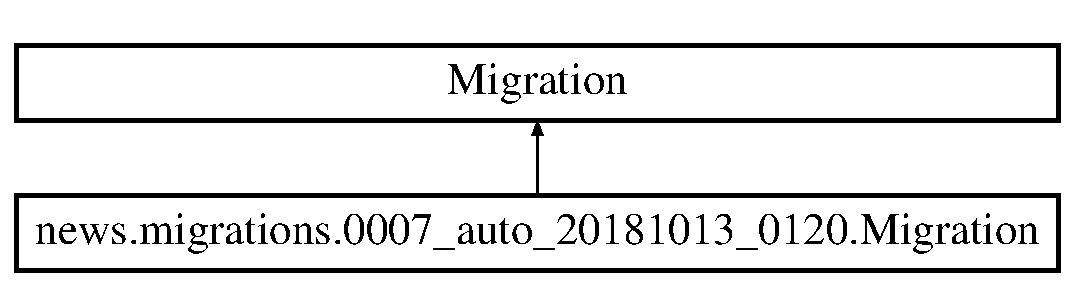
\includegraphics[height=2.000000cm]{classnews_1_1migrations_1_10007__auto__20181013__0120_1_1_migration}
\end{center}
\end{figure}
\subsection*{Static Public Attributes}
\begin{DoxyCompactItemize}
\item 
list \mbox{\hyperlink{classnews_1_1migrations_1_10007__auto__20181013__0120_1_1_migration_a1b2591a8eeaf626e4725684d54a1fdcb}{dependencies}}
\item 
list \mbox{\hyperlink{classnews_1_1migrations_1_10007__auto__20181013__0120_1_1_migration_af1237b52d8a38918f6d7d1ad584aca31}{operations}}
\end{DoxyCompactItemize}


\subsection{Member Data Documentation}
\mbox{\Hypertarget{classnews_1_1migrations_1_10007__auto__20181013__0120_1_1_migration_a1b2591a8eeaf626e4725684d54a1fdcb}\label{classnews_1_1migrations_1_10007__auto__20181013__0120_1_1_migration_a1b2591a8eeaf626e4725684d54a1fdcb}} 
\index{news\+::migrations\+::0007\+\_\+auto\+\_\+20181013\+\_\+0120\+::\+Migration@{news\+::migrations\+::0007\+\_\+auto\+\_\+20181013\+\_\+0120\+::\+Migration}!dependencies@{dependencies}}
\index{dependencies@{dependencies}!news\+::migrations\+::0007\+\_\+auto\+\_\+20181013\+\_\+0120\+::\+Migration@{news\+::migrations\+::0007\+\_\+auto\+\_\+20181013\+\_\+0120\+::\+Migration}}
\subsubsection{\texorpdfstring{dependencies}{dependencies}}
{\footnotesize\ttfamily list news.\+migrations.\+0007\+\_\+auto\+\_\+20181013\+\_\+0120.\+Migration.\+dependencies\hspace{0.3cm}{\ttfamily [static]}}

{\bfseries Initial value\+:}
\begin{DoxyCode}
=  [
        (\textcolor{stringliteral}{'news'}, \textcolor{stringliteral}{'0006\_auto\_20181013\_0120'}),
    ]
\end{DoxyCode}
\mbox{\Hypertarget{classnews_1_1migrations_1_10007__auto__20181013__0120_1_1_migration_af1237b52d8a38918f6d7d1ad584aca31}\label{classnews_1_1migrations_1_10007__auto__20181013__0120_1_1_migration_af1237b52d8a38918f6d7d1ad584aca31}} 
\index{news\+::migrations\+::0007\+\_\+auto\+\_\+20181013\+\_\+0120\+::\+Migration@{news\+::migrations\+::0007\+\_\+auto\+\_\+20181013\+\_\+0120\+::\+Migration}!operations@{operations}}
\index{operations@{operations}!news\+::migrations\+::0007\+\_\+auto\+\_\+20181013\+\_\+0120\+::\+Migration@{news\+::migrations\+::0007\+\_\+auto\+\_\+20181013\+\_\+0120\+::\+Migration}}
\subsubsection{\texorpdfstring{operations}{operations}}
{\footnotesize\ttfamily list news.\+migrations.\+0007\+\_\+auto\+\_\+20181013\+\_\+0120.\+Migration.\+operations\hspace{0.3cm}{\ttfamily [static]}}

{\bfseries Initial value\+:}
\begin{DoxyCode}
=  [
        migrations.RemoveField(
            model\_name=\textcolor{stringliteral}{'blog'},
            name=\textcolor{stringliteral}{'rating\_de'},
        ),
        migrations.RemoveField(
            model\_name=\textcolor{stringliteral}{'blog'},
            name=\textcolor{stringliteral}{'rating\_en'},
        ),
        migrations.RemoveField(
            model\_name=\textcolor{stringliteral}{'blog'},
            name=\textcolor{stringliteral}{'rating\_ru'},
        ),
    ]
\end{DoxyCode}


The documentation for this class was generated from the following file\+:\begin{DoxyCompactItemize}
\item 
news/migrations/\mbox{\hyperlink{0007__auto__20181013__0120_8py}{0007\+\_\+auto\+\_\+20181013\+\_\+0120.\+py}}\end{DoxyCompactItemize}

\hypertarget{classnews_1_1migrations_1_10003__text_1_1_migration}{}\section{news.\+migrations.0003\+\_\+text.Migration Class Reference}
\label{classnews_1_1migrations_1_10003__text_1_1_migration}\index{news.\+migrations.\+0003\+\_\+text.\+Migration@{news.\+migrations.\+0003\+\_\+text.\+Migration}}
Inheritance diagram for news.\+migrations.0003\+\_\+text.Migration\+:\begin{figure}[H]
\begin{center}
\leavevmode
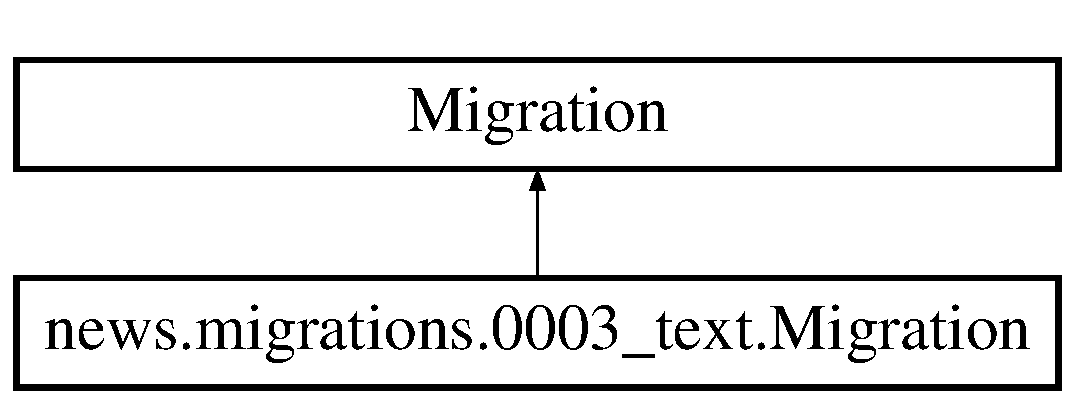
\includegraphics[height=2.000000cm]{classnews_1_1migrations_1_10003__text_1_1_migration}
\end{center}
\end{figure}
\subsection*{Static Public Attributes}
\begin{DoxyCompactItemize}
\item 
list \mbox{\hyperlink{classnews_1_1migrations_1_10003__text_1_1_migration_a6d0db3dbb85d6adb6ffe672d6b5138ca}{dependencies}}
\item 
list \mbox{\hyperlink{classnews_1_1migrations_1_10003__text_1_1_migration_a3cb1f86200fa9c7e658488f99ddb088a}{operations}}
\end{DoxyCompactItemize}


\subsection{Member Data Documentation}
\mbox{\Hypertarget{classnews_1_1migrations_1_10003__text_1_1_migration_a6d0db3dbb85d6adb6ffe672d6b5138ca}\label{classnews_1_1migrations_1_10003__text_1_1_migration_a6d0db3dbb85d6adb6ffe672d6b5138ca}} 
\index{news\+::migrations\+::0003\+\_\+text\+::\+Migration@{news\+::migrations\+::0003\+\_\+text\+::\+Migration}!dependencies@{dependencies}}
\index{dependencies@{dependencies}!news\+::migrations\+::0003\+\_\+text\+::\+Migration@{news\+::migrations\+::0003\+\_\+text\+::\+Migration}}
\subsubsection{\texorpdfstring{dependencies}{dependencies}}
{\footnotesize\ttfamily list news.\+migrations.\+0003\+\_\+text.\+Migration.\+dependencies\hspace{0.3cm}{\ttfamily [static]}}

{\bfseries Initial value\+:}
\begin{DoxyCode}
=  [
        (\textcolor{stringliteral}{'news'}, \textcolor{stringliteral}{'0002\_auto\_20181009\_2006'}),
    ]
\end{DoxyCode}
\mbox{\Hypertarget{classnews_1_1migrations_1_10003__text_1_1_migration_a3cb1f86200fa9c7e658488f99ddb088a}\label{classnews_1_1migrations_1_10003__text_1_1_migration_a3cb1f86200fa9c7e658488f99ddb088a}} 
\index{news\+::migrations\+::0003\+\_\+text\+::\+Migration@{news\+::migrations\+::0003\+\_\+text\+::\+Migration}!operations@{operations}}
\index{operations@{operations}!news\+::migrations\+::0003\+\_\+text\+::\+Migration@{news\+::migrations\+::0003\+\_\+text\+::\+Migration}}
\subsubsection{\texorpdfstring{operations}{operations}}
{\footnotesize\ttfamily list news.\+migrations.\+0003\+\_\+text.\+Migration.\+operations\hspace{0.3cm}{\ttfamily [static]}}

{\bfseries Initial value\+:}
\begin{DoxyCode}
=  [
        migrations.CreateModel(
            name=\textcolor{stringliteral}{'Text'},
            fields=[
                (\textcolor{stringliteral}{'id'}, models.AutoField(auto\_created=\textcolor{keyword}{True}, primary\_key=\textcolor{keyword}{True}, serialize=\textcolor{keyword}{False}, verbose\_name=\textcolor{stringliteral}{
      'ID'})),
                (\textcolor{stringliteral}{'short'}, models.CharField(max\_length=10, verbose\_name=\textcolor{stringliteral}{'L'})),
            ],
        ),
    ]
\end{DoxyCode}


The documentation for this class was generated from the following file\+:\begin{DoxyCompactItemize}
\item 
news/migrations/\mbox{\hyperlink{0003__text_8py}{0003\+\_\+text.\+py}}\end{DoxyCompactItemize}

\hypertarget{classnews_1_1admin_1_1_news_admin}{}\section{news.\+admin.\+News\+Admin Class Reference}
\label{classnews_1_1admin_1_1_news_admin}\index{news.\+admin.\+News\+Admin@{news.\+admin.\+News\+Admin}}
Inheritance diagram for news.\+admin.\+News\+Admin\+:\begin{figure}[H]
\begin{center}
\leavevmode
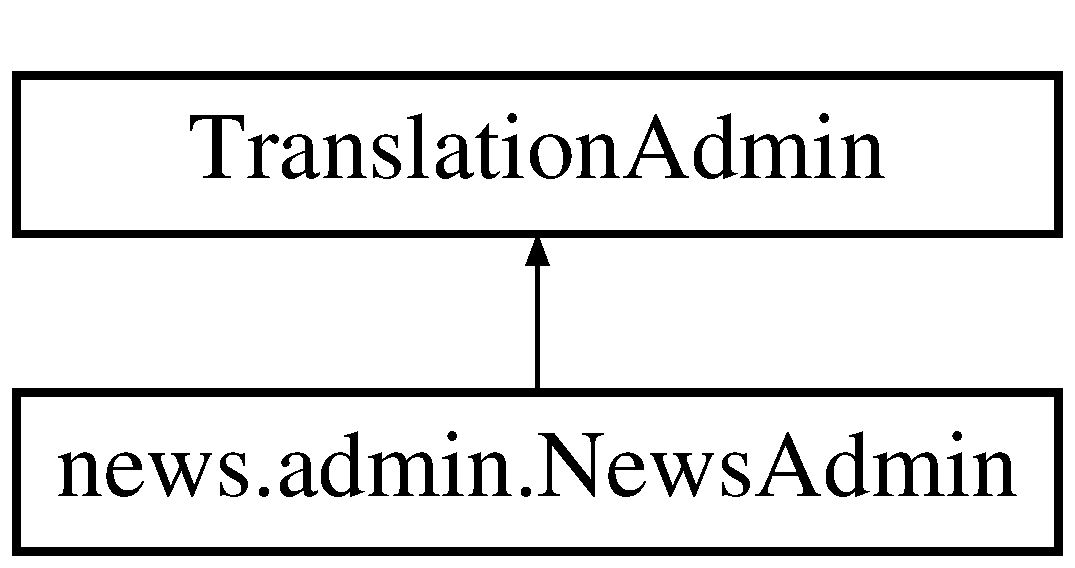
\includegraphics[height=2.000000cm]{classnews_1_1admin_1_1_news_admin}
\end{center}
\end{figure}


The documentation for this class was generated from the following file\+:\begin{DoxyCompactItemize}
\item 
news/\mbox{\hyperlink{admin_8py}{admin.\+py}}\end{DoxyCompactItemize}

\hypertarget{classnews_1_1apps_1_1_news_config}{}\section{news.\+apps.\+News\+Config Class Reference}
\label{classnews_1_1apps_1_1_news_config}\index{news.\+apps.\+News\+Config@{news.\+apps.\+News\+Config}}
Inheritance diagram for news.\+apps.\+News\+Config\+:\begin{figure}[H]
\begin{center}
\leavevmode
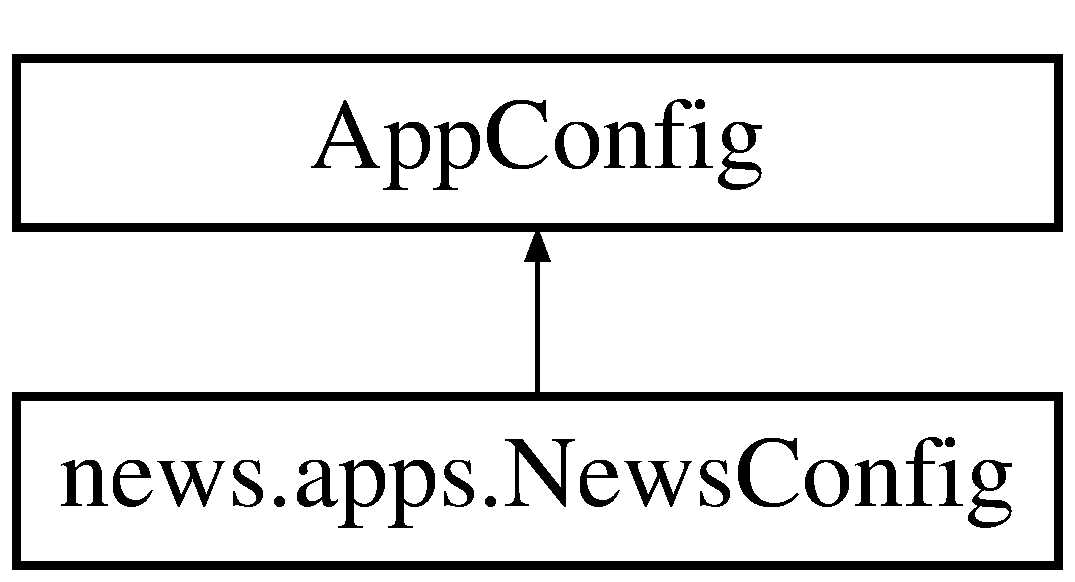
\includegraphics[height=2.000000cm]{classnews_1_1apps_1_1_news_config}
\end{center}
\end{figure}
\subsection*{Static Public Attributes}
\begin{DoxyCompactItemize}
\item 
string \mbox{\hyperlink{classnews_1_1apps_1_1_news_config_a76565ed0ccd338b3e149ea11b729f1c0}{name}} = \textquotesingle{}news\textquotesingle{}
\end{DoxyCompactItemize}


\subsection{Member Data Documentation}
\mbox{\Hypertarget{classnews_1_1apps_1_1_news_config_a76565ed0ccd338b3e149ea11b729f1c0}\label{classnews_1_1apps_1_1_news_config_a76565ed0ccd338b3e149ea11b729f1c0}} 
\index{news\+::apps\+::\+News\+Config@{news\+::apps\+::\+News\+Config}!name@{name}}
\index{name@{name}!news\+::apps\+::\+News\+Config@{news\+::apps\+::\+News\+Config}}
\subsubsection{\texorpdfstring{name}{name}}
{\footnotesize\ttfamily string news.\+apps.\+News\+Config.\+name = \textquotesingle{}news\textquotesingle{}\hspace{0.3cm}{\ttfamily [static]}}



The documentation for this class was generated from the following file\+:\begin{DoxyCompactItemize}
\item 
news/\mbox{\hyperlink{apps_8py}{apps.\+py}}\end{DoxyCompactItemize}

\chapter{File Documentation}
\hypertarget{____init_____8py}{}\section{news/\+\_\+\+\_\+init\+\_\+\+\_\+.py File Reference}
\label{____init_____8py}\index{news/\+\_\+\+\_\+init\+\_\+\+\_\+.\+py@{news/\+\_\+\+\_\+init\+\_\+\+\_\+.\+py}}
\subsection*{Namespaces}
\begin{DoxyCompactItemize}
\item 
 \mbox{\hyperlink{namespacenews}{news}}
\end{DoxyCompactItemize}

\hypertarget{migrations_2____init_____8py}{}\section{news/migrations/\+\_\+\+\_\+init\+\_\+\+\_\+.py File Reference}
\label{migrations_2____init_____8py}\index{news/migrations/\+\_\+\+\_\+init\+\_\+\+\_\+.\+py@{news/migrations/\+\_\+\+\_\+init\+\_\+\+\_\+.\+py}}
\subsection*{Namespaces}
\begin{DoxyCompactItemize}
\item 
 \mbox{\hyperlink{namespacenews_1_1migrations}{news.\+migrations}}
\end{DoxyCompactItemize}

\hypertarget{admin_8py}{}\section{news/admin.py File Reference}
\label{admin_8py}\index{news/admin.\+py@{news/admin.\+py}}
\subsection*{Classes}
\begin{DoxyCompactItemize}
\item 
class \mbox{\hyperlink{classnews_1_1admin_1_1_news_admin}{news.\+admin.\+News\+Admin}}
\item 
class \mbox{\hyperlink{classnews_1_1admin_1_1_blog_admin}{news.\+admin.\+Blog\+Admin}}
\end{DoxyCompactItemize}
\subsection*{Namespaces}
\begin{DoxyCompactItemize}
\item 
 \mbox{\hyperlink{namespacenews_1_1admin}{news.\+admin}}
\end{DoxyCompactItemize}

\hypertarget{apps_8py}{}\section{news/apps.py File Reference}
\label{apps_8py}\index{news/apps.\+py@{news/apps.\+py}}
\subsection*{Classes}
\begin{DoxyCompactItemize}
\item 
class \mbox{\hyperlink{classnews_1_1apps_1_1_news_config}{news.\+apps.\+News\+Config}}
\end{DoxyCompactItemize}
\subsection*{Namespaces}
\begin{DoxyCompactItemize}
\item 
 \mbox{\hyperlink{namespacenews_1_1apps}{news.\+apps}}
\end{DoxyCompactItemize}

\hypertarget{0001__initial_8py}{}\section{news/migrations/0001\+\_\+initial.py File Reference}
\label{0001__initial_8py}\index{news/migrations/0001\+\_\+initial.\+py@{news/migrations/0001\+\_\+initial.\+py}}
\subsection*{Classes}
\begin{DoxyCompactItemize}
\item 
class \mbox{\hyperlink{classnews_1_1migrations_1_10001__initial_1_1_migration}{news.\+migrations.\+0001\+\_\+initial.\+Migration}}
\end{DoxyCompactItemize}
\subsection*{Namespaces}
\begin{DoxyCompactItemize}
\item 
 \mbox{\hyperlink{namespacenews_1_1migrations_1_10001__initial}{news.\+migrations.\+0001\+\_\+initial}}
\end{DoxyCompactItemize}

\hypertarget{0002__auto__20181009__2006_8py}{}\section{news/migrations/0002\+\_\+auto\+\_\+20181009\+\_\+2006.py File Reference}
\label{0002__auto__20181009__2006_8py}\index{news/migrations/0002\+\_\+auto\+\_\+20181009\+\_\+2006.\+py@{news/migrations/0002\+\_\+auto\+\_\+20181009\+\_\+2006.\+py}}
\subsection*{Classes}
\begin{DoxyCompactItemize}
\item 
class \mbox{\hyperlink{classnews_1_1migrations_1_10002__auto__20181009__2006_1_1_migration}{news.\+migrations.\+0002\+\_\+auto\+\_\+20181009\+\_\+2006.\+Migration}}
\end{DoxyCompactItemize}
\subsection*{Namespaces}
\begin{DoxyCompactItemize}
\item 
 \mbox{\hyperlink{namespacenews_1_1migrations_1_10002__auto__20181009__2006}{news.\+migrations.\+0002\+\_\+auto\+\_\+20181009\+\_\+2006}}
\end{DoxyCompactItemize}

\hypertarget{0003__text_8py}{}\section{news/migrations/0003\+\_\+text.py File Reference}
\label{0003__text_8py}\index{news/migrations/0003\+\_\+text.\+py@{news/migrations/0003\+\_\+text.\+py}}
\subsection*{Classes}
\begin{DoxyCompactItemize}
\item 
class \mbox{\hyperlink{classnews_1_1migrations_1_10003__text_1_1_migration}{news.\+migrations.\+0003\+\_\+text.\+Migration}}
\end{DoxyCompactItemize}
\subsection*{Namespaces}
\begin{DoxyCompactItemize}
\item 
 \mbox{\hyperlink{namespacenews_1_1migrations_1_10003__text}{news.\+migrations.\+0003\+\_\+text}}
\end{DoxyCompactItemize}

\hypertarget{0004__delete__text_8py}{}\section{news/migrations/0004\+\_\+delete\+\_\+text.py File Reference}
\label{0004__delete__text_8py}\index{news/migrations/0004\+\_\+delete\+\_\+text.\+py@{news/migrations/0004\+\_\+delete\+\_\+text.\+py}}
\subsection*{Classes}
\begin{DoxyCompactItemize}
\item 
class \mbox{\hyperlink{classnews_1_1migrations_1_10004__delete__text_1_1_migration}{news.\+migrations.\+0004\+\_\+delete\+\_\+text.\+Migration}}
\end{DoxyCompactItemize}
\subsection*{Namespaces}
\begin{DoxyCompactItemize}
\item 
 \mbox{\hyperlink{namespacenews_1_1migrations_1_10004__delete__text}{news.\+migrations.\+0004\+\_\+delete\+\_\+text}}
\end{DoxyCompactItemize}

\hypertarget{0005__blog_8py}{}\section{news/migrations/0005\+\_\+blog.py File Reference}
\label{0005__blog_8py}\index{news/migrations/0005\+\_\+blog.\+py@{news/migrations/0005\+\_\+blog.\+py}}
\subsection*{Classes}
\begin{DoxyCompactItemize}
\item 
class \mbox{\hyperlink{classnews_1_1migrations_1_10005__blog_1_1_migration}{news.\+migrations.\+0005\+\_\+blog.\+Migration}}
\end{DoxyCompactItemize}
\subsection*{Namespaces}
\begin{DoxyCompactItemize}
\item 
 \mbox{\hyperlink{namespacenews_1_1migrations_1_10005__blog}{news.\+migrations.\+0005\+\_\+blog}}
\end{DoxyCompactItemize}

\hypertarget{0006__auto__20181013__0120_8py}{}\section{news/migrations/0006\+\_\+auto\+\_\+20181013\+\_\+0120.py File Reference}
\label{0006__auto__20181013__0120_8py}\index{news/migrations/0006\+\_\+auto\+\_\+20181013\+\_\+0120.\+py@{news/migrations/0006\+\_\+auto\+\_\+20181013\+\_\+0120.\+py}}
\subsection*{Classes}
\begin{DoxyCompactItemize}
\item 
class \mbox{\hyperlink{classnews_1_1migrations_1_10006__auto__20181013__0120_1_1_migration}{news.\+migrations.\+0006\+\_\+auto\+\_\+20181013\+\_\+0120.\+Migration}}
\end{DoxyCompactItemize}
\subsection*{Namespaces}
\begin{DoxyCompactItemize}
\item 
 \mbox{\hyperlink{namespacenews_1_1migrations_1_10006__auto__20181013__0120}{news.\+migrations.\+0006\+\_\+auto\+\_\+20181013\+\_\+0120}}
\end{DoxyCompactItemize}

\hypertarget{0007__auto__20181013__0120_8py}{}\section{news/migrations/0007\+\_\+auto\+\_\+20181013\+\_\+0120.py File Reference}
\label{0007__auto__20181013__0120_8py}\index{news/migrations/0007\+\_\+auto\+\_\+20181013\+\_\+0120.\+py@{news/migrations/0007\+\_\+auto\+\_\+20181013\+\_\+0120.\+py}}
\subsection*{Classes}
\begin{DoxyCompactItemize}
\item 
class \mbox{\hyperlink{classnews_1_1migrations_1_10007__auto__20181013__0120_1_1_migration}{news.\+migrations.\+0007\+\_\+auto\+\_\+20181013\+\_\+0120.\+Migration}}
\end{DoxyCompactItemize}
\subsection*{Namespaces}
\begin{DoxyCompactItemize}
\item 
 \mbox{\hyperlink{namespacenews_1_1migrations_1_10007__auto__20181013__0120}{news.\+migrations.\+0007\+\_\+auto\+\_\+20181013\+\_\+0120}}
\end{DoxyCompactItemize}

\hypertarget{models_8py}{}\section{news/models.py File Reference}
\label{models_8py}\index{news/models.\+py@{news/models.\+py}}
\subsection*{Classes}
\begin{DoxyCompactItemize}
\item 
class \mbox{\hyperlink{classnews_1_1models_1_1_article}{news.\+models.\+Article}}
\item 
class \mbox{\hyperlink{classnews_1_1models_1_1_blog}{news.\+models.\+Blog}}
\end{DoxyCompactItemize}
\subsection*{Namespaces}
\begin{DoxyCompactItemize}
\item 
 \mbox{\hyperlink{namespacenews_1_1models}{news.\+models}}
\end{DoxyCompactItemize}

\hypertarget{serializers_8py}{}\section{news/serializers.py File Reference}
\label{serializers_8py}\index{news/serializers.\+py@{news/serializers.\+py}}
\subsection*{Classes}
\begin{DoxyCompactItemize}
\item 
class \mbox{\hyperlink{classnews_1_1serializers_1_1_blog_serializer}{news.\+serializers.\+Blog\+Serializer}}
\item 
class \mbox{\hyperlink{classnews_1_1serializers_1_1_blog_serializer_1_1_meta}{news.\+serializers.\+Blog\+Serializer.\+Meta}}
\end{DoxyCompactItemize}
\subsection*{Namespaces}
\begin{DoxyCompactItemize}
\item 
 \mbox{\hyperlink{namespacenews_1_1serializers}{news.\+serializers}}
\end{DoxyCompactItemize}

\hypertarget{tests_8py}{}\section{news/tests.py File Reference}
\label{tests_8py}\index{news/tests.\+py@{news/tests.\+py}}
\subsection*{Namespaces}
\begin{DoxyCompactItemize}
\item 
 \mbox{\hyperlink{namespacenews_1_1tests}{news.\+tests}}
\end{DoxyCompactItemize}

\hypertarget{translation_8py}{}\section{news/translation.py File Reference}
\label{translation_8py}\index{news/translation.\+py@{news/translation.\+py}}
\subsection*{Classes}
\begin{DoxyCompactItemize}
\item 
class \mbox{\hyperlink{classnews_1_1translation_1_1_article_translation_options}{news.\+translation.\+Article\+Translation\+Options}}
\item 
class \mbox{\hyperlink{classnews_1_1translation_1_1_blog_translation_options}{news.\+translation.\+Blog\+Translation\+Options}}
\end{DoxyCompactItemize}
\subsection*{Namespaces}
\begin{DoxyCompactItemize}
\item 
 \mbox{\hyperlink{namespacenews_1_1translation}{news.\+translation}}
\end{DoxyCompactItemize}

\hypertarget{views_8py}{}\section{news/views.py File Reference}
\label{views_8py}\index{news/views.\+py@{news/views.\+py}}
\subsection*{Classes}
\begin{DoxyCompactItemize}
\item 
class \mbox{\hyperlink{classnews_1_1views_1_1_blog_view_set}{news.\+views.\+Blog\+View\+Set}}
\end{DoxyCompactItemize}
\subsection*{Namespaces}
\begin{DoxyCompactItemize}
\item 
 \mbox{\hyperlink{namespacenews_1_1views}{news.\+views}}
\end{DoxyCompactItemize}
\subsection*{Functions}
\begin{DoxyCompactItemize}
\item 
def \mbox{\hyperlink{namespacenews_1_1views_a9b0aa87e18d6a69dace52301e34fbfff}{news.\+views.\+my\+\_\+view}} (request)
\item 
def \mbox{\hyperlink{namespacenews_1_1views_a8340d5eecfeb6b527e83164ebf11580b}{news.\+views.\+article}} (request, number)
\item 
def \mbox{\hyperlink{namespacenews_1_1views_a9f55268cd38d1b07e5d941a907d342cc}{news.\+views.\+change\+\_\+lang}} (request, code)
\item 
def \mbox{\hyperlink{namespacenews_1_1views_a6da9b0f94e29b0e9c1a410bfdda103c5}{news.\+views.\+about}} (request)
\item 
def \mbox{\hyperlink{namespacenews_1_1views_a89cc055821d1237b88ca3cf30f78f71f}{news.\+views.\+get\+All}} (request)
\end{DoxyCompactItemize}

%--- End generated contents ---

% Index
\backmatter
\newpage
\phantomsection
\clearemptydoublepage
\addcontentsline{toc}{chapter}{Index}
\printindex

\end{document}
